GoTxn is a transaction system we implemented and verified as the foundation for
DaisyNFS. The goal is to handle crash safety and concurrency for arbitrary
operations within this layer, exporting an interface where transactions appear
to run atomically. Reasoning within a transaction is left to the caller, but
this reasoning is now sequential so it is easier to implement sophisticated and
efficient code on top.

In this chapter we set out the precise specification that GoTxn provides. The
GoTxn implementation is built up in several layers of abstraction. We outline
this implementation and sketch the most interesting parts of the proof. Of
foremost importance is that GoTxn consists primarily of a \emph{journaling
system}, GoJournal~\cite{chajed:gojournal}. The journaling system makes
operations crash atomic but requires the caller to guarantee concurrent
operations do not conflict. GoTxn automatically implements this guarantee using
the two-phase locking algorithm. While two-phase locking involves only a hundred
lines of code or so, it changes the specification dramatically since the caller
gets the illusion of sequential execution without any concurrency control.

\tej{cut the GoJournal intro, make sure to bring back anything important}

%\section{Introduction}


Storage systems, such as file systems, need to be carefully structured
to not lose persistent user data, even in the face of application and
whole-system crashes. They often achieve this \emph{crash safety}
property by delegating writing to storage to a \emph{journaling
system}, which exposes an API for executing an operation such that its
writes appear on disk atomically. The journaling system simplifies
implementing the storage system's logic: to atomically modify a set of
objects, the file system simply writes to them one at a time within a single
journal operation.  The result is that each storage operation is atomic with
respect to crashes.

While a journaling system exposes a simple API, its implementation must address
crash safety and also be concurrent for good performance.
Maintaining correctness in the presence of both concurrency and crashes is
challenging.  For example, in pursuit of performance, journaling systems
often avoid holding locks while performing I/O, but reasoning
about the correctness of such optimizations requires considering what
happens if one thread's disk reads interleave with another thread's
disk writes, and what happens when the system crashes anywhere
during that interleaving.

% \mfk{we should make clear that \txn is a Go package.}
This paper presents \txn, a Go package that provides the first formally verified concurrent journaling
system. To verify \txn, we developed Perennial 2.0, an extension to the Perennial~\citep{chajed:perennial} framework
with several features designed to enable modular reasoning about concurrent, crash-safe systems.
In this work we set a goal of giving
\txn a specification that \emph{reflects the simplicity of using a journal for
crash atomicity}.
\txn can be used by an application like a file system or a key-value
store. As long as the application follows a locking discipline
for its on-disk state, such as per-file locks for a file system, proving the correctness
and crash-safety of that implementation on top of \txn should involve
largely \emph{sequential} reasoning, despite the fact that the application
has multiple concurrent threads and can crash at any time.

Realizing this goal raises two challenges: specifying \txn in a way that makes
application reasoning sequential, and proving \txn's implementation correct. The
specification makes reasoning about an operation sequential with a
\emph{lifting} interface where the proof has an abstraction of a ``checked out''
private fragment of the disk that the operation appears to synchronously modify.
At commit time the private fragment is ``checked in'', at which point it is
durable and can be exposed to other threads. The journal guarantees the
operation is atomic by delaying all writes to commit time, so the developer
should not need to explicitly reason about crash safety until commit time.
Perennial 2.0 supports a new technique called \emph{crash framing} to formalize
the intuition that during an operation the developer need not explicitly
consider crash safety.

The second challenge lies in proving \txn itself.  This is
difficult because we desire modularity to make the system's proof tractable,
which requires giving suitable specifications to the internal interfaces of the system.
While the user-visible interface of \txn is simple, the
internal interfaces of a high-performance journaling system are
hard to specify and fit together.
To address this challenge, Perennial 2.0 contributes \emph{logically atomic crash
  specifications} which enable natural specifications of system layers in terms of
a transition system with
atomic transitions for the public methods.
These specifications include a \emph{crash transition}
to describe what happens to the state of a layer during a crash.
% These specifications both intuitively correspond to atomicity
% and are precise enough
Such specifications make it possible to build upper layers of the system on top without
worrying about implementation details of how atomic transitions are achieved.
This separation of concerns lines up with the modularity in the implementation;
the proof layers divide up the reasoning along the same lines that the
code divides up functionality among Go packages.
% Furthermore, we needed
% to incorporate a \emph{crash transition} into the transition system to specify exactly
% what data can be lost on crash, since some of the internal APIs of \txn buffer
% data in memory before persisting it. \mfk{I don't understand this last
%   sentence. And, I would like to avoid another ``we''}

% The internal API makes it difficult to achieve the desired strong
% specification of atomic transactions. The reason the strong specification
% holds is due to the use of locks to protect disk-object ownership. Under
% these ownership assumptions, the journaling system can prove that the
% internal APIs behave atomically with a single logical commit point.

% We implemented \sys on top of Perennial~\cite{chajed:perennial}, a
% concurrent crash-safe verification framework.  We then implemented
% \txn and used \sys to formally specify and prove its correctness and
% crash safety; in the process of doing so we found one design bug that
% was not caught by unit tests (\S\ref{sec:eval:bugs}).

The contributions of this paper are (1) \txn, a concurrent
journaling system with a machine-checked proof of correctness and
crash-safety; (2) the Perennial 2.0 framework, with extensions to the original
Perennial framework that enable modularity and crash-free reasoning on top of \txn;
and (3) \simplenfs, a verified core of an NFSv3 file server built on
top of \txn.

Although \txn is advanced enough to support a high-performance NFS
server, it has some limitations.  \txn's internals (code and proof)
support deferred durability, but for simplicity, \txn's top-level
specification requires applications to immediately flush committed
journal operations, which is sufficient to prove \simplenfs.  \txn is also
less general than JBD2 (e.g., \txn does not support floating commit
blocks), and less general than database transaction systems (e.g.,
\txn does not support undoing journaled operations).

%%% Local Variables:
%%% mode: latex
%%% TeX-master: "paper.tex"
%%% End:

\section{GoTxn's specification}

At a high level, GoTxn's specification says that transactions execute
atomically. The way this is stated formally is by considering an arbitrary
caller, a program that has transactions using the GoTxn API. Then correctness is
defined by relating this executable code to an abstract, specification program,
a version of the caller code where the GoTxn methods are treated as primitives.
An important aspect of GoTxn is that the specification program is defined using
an atomic block around each transaction, whose semantics is to run the body
without interleaving other threads.

Before we can get to defining these specification programs, we first set up
\emph{refinement}, which is the relationship between the code and spec.
Abstractly, refinement from a code program to
a specification program says that the behaviors of the code are a subset of the
behaviors of the specification.
To define refinement we need to be more precise about what a program is and how it
executes. We
write $p : \gooselayer{X}$ to say $p$ is a Go program written using operations
from layer X, where X is one of NFS, Txn, or Disk.
Layer operations are always atomic transitions in a state machine. In the
NFS layer, the NFS operations behave according to the NFS state machine
described previously in \autoref{sec:soundness} and defined formally in Dafny.

The Txn layer is specified in both Coq where it is part of GoTxn's correctness
theorem and in Dafny where it appears as an assumption. The Disk transition
system is formalized in Coq as part of the GoJournal proof, and assumes reads
and writes of 4KB blocks are atomic. Each layer includes concurrent threads that
interleave layer operations, basic heap operations on pointers, slices, and
maps, and computation on primitives like integers and structs.

Refinement relates two programs in terms of their visible behavior, which we
will use to connect code written against the transaction system to the
executable code that runs on a disk. When refinement talks about the behavior of
a program, we will take this to mean the network behavior that DaisyNFS has at
the top level, from interacting with NFS clients.

\begin{definition}[Refinement]
  An implementation program $p_{c}$ refines a specification program $p_{s}$,
written $p_{c} \refines p_{s}$, if whenever there are initial states
$\sigma_{s}$ and $\sigma_{c}$ satisfying $\mathrm{init}(\sigma_{s}, \sigma_{c})$
and $p_{c}$ can execute from $\sigma_{c}$ and produce a trace of network I/O
$tr$, then $p_{s}$ can execute from $\sigma_{s}$ and produce the same trace
$tr$.  Execution might involve crashing and restarting a program (potentially
multiple times), wiping out any in-memory state after each crash.
  \label{def:refinement}
\end{definition}

The intuition behind the notation $p_{c} \refines p_{s}$ is that the set of
behaviors of $p_{c}$ (the set of traces of network I/O $tr$) is a subset of the
behaviors of $p_{s}$. Whenever we state $p_{c} \refines p_{s}$ we leave implicit
a definition of initial states $\mathrm{init}(\sigma_{s}, \sigma_{c})$, which
will generally say both states are all zeros and of the same size.

\subsection{Correctness theorem for the transaction system}
\label{sec:proof:txn}

The \cc{Txn} layer semantics serves as the interface between the Perennial and Dafny
proofs.  It specifies that transactions are atomic in the sense that code
enclosed within a transaction \cc{Begin} and \cc{Commit} happens all at once (or
does nothing, if \cc{Abort} is executed), without interleaving of steps by other
threads.

We define the correctness of the transaction system's implementation as a
\emph{program refinement}.
To set up this specification, consider a program $p : \gooselayer{Txn}$ that
uses transactions.
To run $p$, it is combined with the transaction-system implementation, producing
a program $\mathrm{link}(p, \txncode) : \gooselayer{Disk}$ that can be run on
top of a disk.
Transactions in the linked program continue to have the expected atomic
behavior, so long as transaction code in $p$ follows certain restrictions, such
as not accessing shared state outside the journal system.  We write
$\mathrm{safe}(p)$ to mean $p$ is ``safe'' in the sense that it follows these restrictions.

% At a high level of abstraction, the main difficulty is to give a specification
% for the transaction system, which we do in several steps:
%
% \begin{enumerate}
%   \item First, we define an arbitrary Go program running on top of
%         the transaction system. For reasons we will explain shortly we will use
%         $p : \gooselayer{Txn}$ for such a program. To run such a program it
%         first needs to be linked with the transaction system implementation,
%         producing a program denoted $\mathrm{link}(p, \txncode)$.
%   \item The second idea is to say what the semantics of a program
%         $p : \gooselayer{Txn}$ is. Transactions are atomic in this semantics in
%         that the whole transaction transitions at once, without interleaving
%         other threads. The program can issue reads and writes within a
%         transaction, and they follow a simple state machine.
%   \item The final idea is to define ``safe'' programs $\mathrm{safe}(p)$, those
%         that follow the restrictions of the transaction system. The
%         specification only applies to safe programs.
% \end{enumerate}

The correctness of the transaction system is summarized by the following theorem:

\begin{theorem}
  The transaction system's implementation $\txncode$ is a program refinement, meaning for
  all $p : \gooselayer{Txn}$, if $\mathrm{safe}(p)$, then
  $\mathrm{link}(p, \txncode) \refines p$. The definition of
  $init(\sigma_{s}, \sigma_{c})$ in this refinement relates an all-zero physical
  disk to an all-zero transactional disk of the same size.
  \label{thm:txn}
\end{theorem}

\autoref{thm:txn} is stated in Coq and has a fully mechanized proof in Perennial.
What it says is that if a program is safe, the program linked with the
transaction system always behaves as if its transactions were atomically
accessing a transactional disk logically maintained by the transaction system.
The definition of safety formalized in Coq requires that code within a
transaction not access any shared memory outside of the transaction layer; other
than that, transactions are permitted to issue reads, writes, and do other
computation. Safety also requires that transactions follow the preconditions of
the \cc{Read} and \cc{Write} operations, which require a discipline of accessing
each object with a fixed size. Finally, safe programs can only \cc{Abort} or
\cc{Commit} a given transaction once. The notion of safe program will be
important when linking this proof with the Dafny proofs, since the transaction
system's proof only applies to a safe caller.

In the Coq development, \autoref{thm:txn} uses Goose~\cite{chajed:goose-coqpl}
to translate the transaction system's Go implementation into a model in Coq that
Perennial supports.

%To the best of our knowledge, \txn is the first verified concurrent,
crash-safe journaling system. The verification of \txn builds on a
large body of previous work, as described in the rest of this
section.

\subsection{Perennial 2.0 vs Perennial 1.0}

The verification approach we take is based on a new version of our earlier
Perennial~\cite{chajed:perennial} framework, so we draw a contrast between the
two here. The new implementation is
conceptually similar in that it supports reasoning about concurrency and
crash-safety, it is implemented on top of the
Iris~\citep{jung:iris-jfp,jung:iris-1} concurrency verification system,
and it uses Goose~\cite{chajed:goose-coqpl} to enable verification of Go
programs by translating them into a model in Perennial 2.0.
However, to make verification of \txn feasible, we had to re-write many core parts of the framework.
To clarify which framework is being referenced we will write Perennial 1.0 for the
original framework and Perennial 2.0 for the new one in this section, in order
to highlight the new features Perennial 2.0 supports. The rest of the paper
generally refers only to Perennial 2.0.

%Perennial 1.0 supported verifying Go programs with a system called
%Goose~\cite{chajed:goose-coqpl} that translates Go into a model in Perennial.
%Perennial 2.0 also comes with a new version of Goose that supports the new
%verification infrastructure and extends translation to cover additional features
%in Go used in \txn.



Some of Perennial 2.0's features are needed to support the \txn top-level
specification and enable verification on top of this interface. The reason this
problem is complicated is because the journal does not make operations
automatically atomic but requires the caller to correctly manage ownership, and
Perennial 1.0's refinement specifications do not give a good way to talk about
ownership. The top-level specification of \txn relies on \emph{crash
framing}~(\autoref{s:design:crashframe}) and \emph{crash-aware
locks}~(\autoref{s:design:crashlock}) to enable application proofs that reason
about ownership of durable data.

Perennial 2.0 also scales to a larger system than the mail server verified in
Perennial 1.0. One of the challenges with the larger system is that it has many
internal layers that need their own specifications, so that the proof can be
carried out modularly. Normally a separation logic or refinement-based
specification would be sufficient, but we need internal specifications that capture
the crash and concurrent behavior of each internal library. To that end
Perennial 2.0 incorporates a new specification style which adds \emph{crash
atomicity} to the logically atomic specification styles developed in earlier
work~\citep{jacobs:logatom,svendsen:hocap,pinto:tada}. Modularity in the proof
was necessary to scale verification to
all of \txn's performance optimizations and concurrency.
At the same time, \txn's specification allows
the proof of \simplenfs to mostly avoid reasoning about crashes.

%% The specification for the simple NFS server is based on closely reading RFC
%% 1813~\cite{RFC:1813}, which defines the NFSv3 API in English prose. We do not
%% attempt to formalize all allowed behaviors in the specification, but did attempt
%% to write a formal specification in Coq which would meet the prose specification.
%% \mfk{maybe say we have some confidence in our formal spec, because
%%   \simplenfs can be mounted and used by a linux client.}

%% \joe{talk about JBD2 here}

%% Lifting and disk-object ownership are
%% new techniques that would not more complicated in Perennial due to the
%% need for leases. Perennial does demonstrate a complex example that
%% requires recovery helping to prove correct; our framework does not
%% support this pattern, but we did not need it to prove \txn or the file
%% system since no helping is involved.

%% The most obvious difference to Perennial is the difference in verified artifact:
%% we prove \txn, a \gotxnLOC-line, high-performance transaction system with interesting
%% crash safety and concurrency challenges, along with a \simplenfsLOC-line NFS server using
%% it; Perennial verified a 150-line mail server. Besides simply having much more
%% code, \txn is verified in several modular layers, with four internal APIs, and
%% then we use the specification to verify an application. Perennial did not
%% explain or demonstrate a modular verification story; our contribution of
%% logically atomic crash specifications allows us to scale verification to this
%% larger system by specifying internal APIs, which are more complex than the
%% client-visible one.

%% Perennial did not include explicit crash conditions, instead carrying out all
%% crash reasoning using an invariant. This works for small examples but is
%% inconvenient for modular verification. We instead build on a framework that uses
%% Iris but augments Hoare logic specifications with a crash condition, in the
%% style of FSCQ's Crash Hoare Logic, but extended to support concurrency.

% \subsection{Related verification efforts}

\subsection{Related verification frameworks}

\paragraph{Crash-safe systems.}

% Perennial 2.0's atomic crash specifications enable \txn to formalize the crash behavior
% of a layer in a lightweight fashion---that is, promising that a layer does not
% expose any unexpected intermediate states after a crash.
Any crash-safe system
must reason about the possible states after a crash, and several prior works
have formalized this in different ways for \emph{sequential} crash-safe systems.
FSCQ~\cite{chen:fscq,chen:dfscq} uses Crash Hoare Logic (CHL) to specify crash
behavior through a crash condition, which describes the state of a system if a
crash happens during execution of a function. Alternatively, a number of systems
verify crash safety using refinement
reasoning~\cite{sigurbjarnarson:yggdrasil,ernst:crash-refinement-asms,chajed:argosy,hance:veribetrkv},
but none support the combination of concurrency and crash-safety.

% However, refinement-based proofs can require additional layers for proof purposes
% that do not correspond to modules in the original code.

% However, refinement based proofs can be heavy-weight because they require
% formalizing the entire set of operations that can be performed at every layer of
% a refinement proof (including logically orthogonal operations like allocating
% memory, accessing data structures, and calling other libraries).
% \ralf{I don't understand the last sentence. It seems to be specifically about CSPEC, not refinement proofs in general?}

Although they are not concurrent, some of these systems address other
aspects of performant storage systems that are not found in \txn.
DFSCQ~\cite{chen:dfscq} verifies a high-performance file system built
on top of a logging system with asynchronous disks and log-bypass
writes, which are challenging optimizations that \txn does not
support. VeriBetrKV~\cite{hance:veribetrkv} verifies a key-value store
based on B\textsuperscript{$\epsilon$} trees, a data structure that also underlies BetrFS~\cite{jannen:betrfs}. \txn
and \simplenfs use simple data structures;
the challenge lies in accounting for concurrent accesses.
%where the challenge is concurrent access.
% concurrent access to these structures.

% The proof technique uses refinement between layers
% in a way that is lighter-weight and more flexible than in CSPEC,a and
% additionally uses the crash guarantees of one layer to prove the crash
% guarantees of a higher layer. VeriBetrFS is implemented in Dafny, which has
% tight integration with Hoare logic; this makes it easier to use but also harder
% to extend, particularly with concurrency. In Coq the program logic is not
% built-in, which gives the flexibility to implement a new logic (as FSCQ did) or
% to extend an existing one (as we do on top of the Iris program logic).

\paragraph{Concurrent systems.}

In addition to specifying behavior at intermediate crash points, Perennial 2.0's
specifications describe the atomic commit points of concurrent operations. A
range of verification techniques have been used to address this kind of
challenge in concurrent systems. AtomFS~\cite{zou:atomfs} uses a framework
called CRL-H (concurrent relational logic with helpers) to verify a concurrent
in-memory file system implemented in C. Refinement-based systems such as
CSPEC~\cite{chajed:cspec}, Armada~\cite{lorch:armada}, and Concurrent
CertiKOS~\cite{gu:certikos-ccal} typically prove that a function implements an
atomic operation at a more abstract layer.
However, in \txn, many internal APIs provide operations that are only atomic if
the caller owns some data. This kind of conditional atomicity is easy to express
in Perennial 2.0 using separation logic, but hard to express
as a precondition in a transition system.
% Additionally, as with using refinement for crash-safety reasoning, refinement-based approaches often introduce extra layers for proof purposes. On the other hand, proofs of refinement between
% layers in an SMT-based system like Armada are automated, while proofs are
% interactive in Perennial 2.0.

% Armada~\cite{lorch:armada} also verifies C code but uses a different approach
% based on several layers of refinement between levels, which are progressively
% more abstract versions of the code. Neither of these frameworks
% supports crash-safety guarantees, and neither supports modular verification of a
% lower-level layer independently of upper layers that use it.


\paragraph{Concurrent, crash-safe reasoning.}

Program logics other than Perennial
have been developed for formal reasoning about concurrent, crash-safe systems.
Fault-Tolerant Concurrent Separation Logic (FTCSL)~\cite{ntzik:faults} extends
the Views~\cite{dinsdale:views} concurrency logic to incorporate crash-safety.
POG~\cite{raad:pog} is a program logic for reasoning about the interaction of
x86-TSO weak-memory consistency and non-volatile memory.
Neither logic has a mechanism for modular proofs of layers,
which we found essential to scale verification to a system of \txn's
complexity. Both are restricted to pen-and-paper proofs, whereas both Perennial
1.0 and 2.0 have machine-checked proofs.

A specification called the Push/Pull model of
transactions~\cite{koskinen:pushpull} is similar to the \emph{lifting} technique
in the journal system's specification~(\autoref{s:design:lifting}) --- the core
problem addressed is that a journal operation atomically modifies a small number
of objects, but other objects can change between the start of the operation and when
it commits. The Push/Pull model also discusses reasoning on top of the
specification, using Lipton's reduction~\cite{lipton:movers} rather than
separation-logic ownership to handle concurrency. However that work is about
on-paper specifications and proofs, while we also prove an implementation meets
our specification and proved \simplenfs on top.

\section{Implementing GoTxn}
\label{s:gotxn:impl}

\begin{figure}
  \centering
  \small
  \begin{tabular}{ll}
    \toprule
    \textbf{Layer} & \textbf{Description} \\
    \midrule
    \scc{txn} & Concurrency control using two-phase locking \\
    \scc{jrnl} & In-memory buffered object operations \\
    \scc{obj} & Journaling sub-block writes \\
    \scc{wal} & Whole-block write-ahead logging \\
    \scc{circ} & On-disk circular log data structure \\
    \midrule
  \end{tabular}
  \caption{The layers in the GoTxn implementation.}
  \label{fig:gotxn-layers}
\end{figure}

The transaction system is structured into several layers, as shown in
\cref{fig:gotxn-layers}. At a high level, three of the abstractions are useful
to understand the overall structure: the \scc{wal}, the \scc{jrnl}, and finally
the top-level \scc{txn}. The first useful abstraction is the
write-ahead log, which behaves like a disk with an atomic multiwrite operation.
Reads and writes still operate on 4KB blocks, but a multiwrite appears to update
multiple disk blocks simultaneously even if the system crashes. Next, the
\scc{jrnl} layer implements \emph{journaling}, persisting a whole operation with
reads and writes to disk atomically. Concurrent operations must access disjoint
addresses for safety; concurrency control is left to the caller in this layer.
Operations can manipulate objects smaller than a block (``sub-block'' objects),
which improves concurrency by making more operations disjoint. Finally, the
\scc{txn} layer exports the complete transactional interface in
\cref{fig:txn-api}. This layer implements automatic concurrency control so that
the caller can freely read and write any addresses.

The write-ahead log is implemented by organizing the disk into a small,
fixed-size circular buffer and a remaining data region. Data is first atomically
\emph{logged} to the circular buffer and then eventually \emph{installed}
to the data region, to free space in the circular buffer. Reads first go through
the circular buffer (which is cached for efficiency) and then access the data
region.

The object system maintains a list of buffers of data read or written by each journal operation.
Reads first check the write-ahead log's cache since
they must observe committed operations. To commit, the object
layer gathers all the dirty buffers and submits them as a multiwrite to the
write-ahead log. To allow reading and writing objects that are smaller than a
block, the object layer assembles these into block writes by doing a
read-modify-write sequence.
%if a block isn't completely overwritten within an operation.

Because disk writes are slow, for good performance the journal executes many
tasks in parallel. Committing new journal operations in memory, logging operations
from memory to disk, waiting for operations to be made durable, and
installing logged writes all happen concurrently.  Concurrency ensures that
in-memory operations
need not wait for any in-flight disk reads or writes, and that many
disk reads and writes can happen at the same time.  Finally, to reduce the
number of disk writes, the write-ahead log implements two optimizations.
Multiwrites are combined and written
together (``group commit''), and if they update the same disk
block multiple times, only the most recent update of that disk block is
written to the log (``absorption''). Concurrency makes these optimizations
useful even for synchronous operations, which can be committed together and
absorbed if they are issued concurrently.

Concurrency in the write-ahead log complicates not just its internals but also
reasoning about the multiwrite abstraction built on top. One difficulty is that
reading requires checking the log's in-memory cache and then falling back to the disk,
but the disk read happens without a lock. If a multiwrite commits after the read
misses in the cache, then the disk read will not observe the latest value. The
write-ahead log specification specifies that reading the installed value might return an
old view of the disk, and the object layer can handle this weak specification with
an invariant that guarantees the object being read has not been modified since
that old view.

The object layer implements sub-block access on top of the write-ahead
log's block-level multiwrites. Objects accessed by an operation must be locked,
so supporting fine-grained access is necessary to allow operations to run
concurrently even if they happen to access the same disk block. For example, a
file system might pack inodes into a block, and locking an inode should not
prevent concurrent operations for other inodes in the same block. The
object-layer implementation is able to execute reads and writes during an
operation without any additional locks, but something more is needed to commit.
Imagine a situation where between reading some disk block and writing it an
unrelated object was modified in the same block; committing the modified block
would overwrite the concurrent modification, losing data. The code addresses
this with a global commit lock that prevents concurrent modifications while
reading the blocks to be written.

The \scc{jrnl} layer implements a journaling system which gives the caller a
useful abstraction over the disk that makes it easy to update the disk in a
crash atomic way but which requires that the caller implement appropriate
concurrency control. The \scc{txn} layer automatically implements the required
concurrency control; this isn't much code beyond the journal, but it does
dramatically change the specification since the caller sees any sequence of
reads and writes as atomic both with respect to threads and crashes without
having to implement any locking.

Journaling makes writes atomic on crash. To make transactions appear atomic
(also known as \emph{serializability}), we use two-phase locking on top of
journaling. This algorithm acquires a lock on each address the first time it is
used in a transaction. Writes are buffered locally until commit time, at which
point they are written atomically using the journaling system. Finally all the
locks are released, exposing the transaction's effects to subsequent
transactions.

% The implementation of the write-ahead log and transaction management is
% complicated primarily because of a highly concurrent implementation. Without
% concurrency, the implementation and specification
% would be similar to the logging system of FSCQ, but a file-system built on top
% would also get little performance benefit from multiple cores. In the evaluation
% we show this loss of performance in a version of \txn's code with its
% concurrency disabled \tej{forward reference and maybe some numbers}.

%%% Local Variables:
%%% mode: latex
%%% TeX-master: "paper.tex"
%%% End:

%% indexing disk generations

% And using its specs reads a little clunky to me -JDT
%\section{Specifying \txn and using its specs}

\section{Specifying GoJournal}
\label{s:design}

%% This section walks through the \txn specification as well as how an application
%% proof uses it to prove linearizability.  We use the simple NFS server and its
%% Write operation as an example to make things more concrete.

%% The idea for code is that the transaction system makes linearizability easy by
%% wrapping everything up in a transaction. The specification realizes this for the
%% proof. \tej{more to say here for context}

%% The high-level flow for the Write transaction is seen in \cc{NFS3_WRITE}:
%% the code starts a transaction with \cc{Begin}, then runs
%% \cc{NFS3_WRITE_locked} within a critical section around the file lock.
%% \cc{NFS3_WRITE_locked} consists of \cc{NFS3_WRITE_wp} --- which
%% prepares the \cc{op} with the buffered writes needed to implement the RPC ---
%% followed by a call to \cc{Commit(true)} to finally make the transaction durable.

\tej{Bunch of work in this section. First explain why this layer is needed in
GoTxn, and second less emphasis on a caller since the spec is only used once
to prove a generic transaction correct.}

\tej{some of the GoJournal paper's motivation (about the difficulty of capturing
the crash atomicity of a journal) do apply to this section, and need to be
introduced locally since the chapter is otherwise about a transaction system}

The goal of \txn's specification is to support convenient reasoning about atomic
operations, like the NFS \scc{write} implementation in \autoref{fig:nfswrite} and \autoref{fig:write}.
In this section we walk through how the specification
guarantees atomicity for the caller without forcing the caller to do
much application-specific reasoning about concurrency or
crashes.

The key to this specification is tracking resources, like the disk blocks making up a
file, as they flow through the steps of the proof. We start by reviewing how
separation logics like Perennial represent these resources, and how
specifications in the logic track logical \emph{ownership} of
resources~(\autoref{s:design:rep}). The specification for \txn introduces
resources that distinguish between a journal operation's local view of an object and
the durable, on-disk representation; obtaining either resource
requires the caller to use correct synchronization, as required by the journal's
implementation. \emph{Lifting} provides a
way to translate
a locked object from its on-disk view to a local view within the operation~(\autoref{s:design:lifting}).
While preparing a journal operation, reads and writes modify the local
view~(\autoref{s:design:read-write}). Finally, committing an operation writes
its updates to disk, so the specification asserts that the local
view becomes a view over durable state.

To take full advantage of the durable and operation-local views of
journal objects, the proof of \scc{Write} uses two new techniques introduced by
Perennial 2.0: crash-aware locking~(\autoref{s:design:crashlock}) and crash
framing~(\autoref{s:design:crashframe}). With these techniques, the proof of
\cc{NFS3_WRITE_op} uses entirely sequential reasoning for preparing the
journal operation, even though concurrent operations might write to disk and its
disk writes are buffered rather than synchronous.
Finally, \autoref{s:design:summary} summarizes how the proof
techniques combine to prove correctness and crash-safety for the NFS \scc{write}
example.

%% This property is sometimes called linearizability,
%% and in this paper we will informally use the term ``linearization point'' to
%% refer to a point after which the operation has logically occurred, meaning other
%% threads will observe its effect.

\subsection{File representation}
\label{s:design:rep}

First, in both designing the code and writing the proof, the NFS server must
establish a disk layout to arrange its data in terms of disk objects. The disk
layout is expressed using a separation-logic \emph{representation invariant}, a
predicate which connects the logical (specification-level) contents of files to the objects (inodes and
blocks) that encode those files.

%  From a
% user's perspective looking at the file system, its state is a collection of
% files named by inode number, where a file is a list of bytes. Internally, in the
% file system, a file with inode number $i$ is stored as a metadata object with
% the file's size and the address of its (single) data block. The proof maintains
% a representation invariant that connects the abstract state of a file seen by
% users to the physical representation in terms of metadata and data.

Representation invariants over the state of the journal use a
``points-to predicate'' $a \mapsto o$, which serves two purposes: it asserts
that the address $a$ (of type \cc{Addr}) contains an object $o$ (which is
represented by the \cc{*Buf} type in the API), and it represents exclusive
\emph{ownership} over the address~$a$. When a thread has $a \mapsto o$ in its
precondition, ownership allows the proof to assume that the value at address $a$
does not change until the thread gives up ownership, and that it will not be
read by other threads.  Locks help threads transfer ownership so a thread only
retains exclusive ownership during a critical section.

The \simplenfs proof connects each file to its representation with the following
representation invariant:
%
\begin{align*}
  &\cc{file_rep}(i, \mathit{data}) \triangleq \exists \mathit{meta}, \exists \mathit{blk}, \\
  &\quad i \mapsto \mathit{meta} \sep \mathit{meta}.\cc{blkno} \mapsto blk \land \phantom{} \\
  &\quad \mathit{meta}.\cc{size} = \cc{length}(\mathit{data}) \land \cc{prefix}(\mathit{data}, \mathit{blk})
\end{align*}

Informally the representation invariant says the file $i$ with logical contents $\mathit{data}$ is represented by some
metadata $\mathit{meta}$ stored at the inode number $i$ and a data block at
$\mathit{meta}.\cc{blkno}$. It then says the file's bytes are a
$\mathit{meta}.\cc{size}$-length prefix of the data block.

This definition uses the separating conjunction $P \sep Q$ (pronounced ``$P$ and
separately $Q$''), which says that two predicates hold over disjoint state.
%\ralf{It mixes separating and regular conjunction... wouldn't it be easier to use separation conjunction throughout?}
For example, this asserts the inode and its data block are stored
separately. To initialize the system the caller must prove that the
\cc{file_rep} predicates hold separately for each file, that is,
$\cc{file_rep}(1, \mathit{data}_1) \sep \cc{file_rep}(2, \mathit{data}_2) \sep \cdots$. Here the
separating conjunction asserts files are represented disjointly, so that when a
thread modifies one file it is guaranteed not to affect data in other files.

\subsection{Lifting}
\label{s:design:lifting}

\newcommand{\bufobjDurable}{\cc{durable_pred}\xspace}

The key idea of \txn's specification is to consider two view of the disk: a
conceptual in-memory view that a buffered journal operation observes, as well as
an on-disk view that reflects what would be on disk after a crash. Parts of both views are constantly changing as
other threads commit operations concurrently, so we use separation logic to
define a local view that contains only objects locked by and involved in a
journal operation. Because the journal operation logically owns these objects, the caller
can use sequential reasoning---disk objects have the same value throughout---and can commit all of the objects written in the operation at
the end without fear of interfering with concurrent journal operations. The
specification makes this informal reasoning concrete using \emph{lifting}, which
we use to refer to this strategy of transferring ownership to and from the
on-going operation.

To do anything with the journal, a thread must first \cc{Begin} an atomic operation:
\hypertarget{tgt:begin-spec}{}
%
\begin{align*}
  \hoareV{\TRUE}{\cc{Begin}()}{\Ret{op}
    \cc{is_op}(\mathit{op}) \sep
    \bufobjDurable(\mathit{op}, \TRUE)}
   %\tagH{BeginSpec}
\end{align*}

The specification above is a Hoare triple for the \cc{Begin()} function. It says
that executing \cc{Begin()} starting with its precondition (in this case $\TRUE$) will run
without errors and if it terminates it will return $\mathit{op}$ along with the
postcondition, namely $\cc{is_op}(\mathit{op}) \sep \bufobjDurable(\mathit{op}, \TRUE)$.
The \cc{is_op} part of the post-condition simply says that $\mathit{op}$ is a
valid \cc{*Op} object. The $\bufobjDurable(\mathit{op}, \TRUE)$ clause is what tracks the
on-disk data ``underneath'' a journal operation, which would be left behind if the
operation aborted; since the operation starts out with an empty local view,
it starts out with no on-disk footprint, written as $\TRUE$.

%Before we can describe lifting, we need a way to talk about the logical state of
% the journal and the local view from within a transaction.

The different views of a journal operation are tracked using \emph{ghost state} in Iris.  Ghost state is separate from
the physical state of the program---the contents of memory and disk---and is
only manipulated by the proof. The journaling system's proof introduces ghost
state for durable state of the system, including an $a \mapsto_{d} o$ predicate
for ownership over individual objects. Note that an object is expressed through
ghost state because the block holding the object might be located in the on-disk
log or in the data region, and ownership of an object says nothing about other
objects in the same disk block.

The proof also introduces a similar $a \mapsto_{\mathit{op}} o$ predicate for the local
view of operation \cc{op}, and it is this ownership that is needed for reads and
writes. A caller obtains these predicates with a logical operation we call
\emph{lifting} that converts ownership of $a \mapsto_{d} o$ into $a \mapsto_{\mathit{op}} o$, granting the
ability to read and write.

\tej{lifting between disk/txn is still important, but lifting of predicates is
irrelevant to GoTxn}

To make it easier to work with lifting, the specification allows lifting an
entire \emph{predicate} $P$ and transforms all of its points-to facts
simultaneously, which we denote this paper denotes by switching subscripts. For
example, we re-use
the definition $\cc{file_rep}$ from \autoref{s:design:rep} for both a file laid
out on disk and a file as owned by a journal operation, which we denote with
$\cc{file_rep}_{d}$ and $\cc{file_rep}_{\mathit{op}}$ respectively. The specification
for lifting a generic predicate $P$ is:
%
\begin{align*}
  \hoareV{P_d \sep \bufobjDurable(\mathit{op}, Q_d)}{\SKIP}{P_{\mathit{op}} \sep \bufobjDurable(\mathit{op}, P_d \sep Q_d)}
\end{align*}

Since lifting is purely logical (it only modifies ghost state), we
write it as a Hoare triple for a no-op, much like how Dafny and \fstar lemmas
are simply methods with pre- and post-conditions but no code~\cite[\S 12.2.3]{dafny-refman}.%
\footnote{In case the reader is already familiar with Iris, these Hoare triples represent
what is usually called a ``view shift'' in Iris.}
The outcome of lifting is to expand the memory covered by the journal operation to
incorporate $P_{d}$. Observe that \bufobjDurable is expanded to ``snapshot''
$P_{d}$, which tracks that if the operation were to abort or crash, the
durable $P_d$ that we started with would still hold.  The on-disk values
do not change over the course of a buffered journal operation (as expected, since these are
in-memory writes). The key part of the postcondition, however, is $P_{op}$: the
$a \mapsto_{op} o$ predicates within $P_{op}$ (e.g., the
$i \mapsto_{\mathit{op}} \mathit{meta}$ within $\cc{file_rep}_{\mathit{op}}(i, \mathit{data})$)
give the caller
the right to read and write objects from within the operation, as we will see
in~\autoref{s:design:read-write}.

% The ghost state involved in defining the $a \mapsto_{\mathit{op}} o$ predicate
% is somewhat subtle in order to implement lifting: the proof must track that
% ownership of this predicate guarantees that the on-disk value of address $a$
% remains $o$.

\subsection{Reads and writes}
\label{s:design:read-write}

The specification for \cc{OverWrite} describes the effect of writing to the
local memory of a buffered journal operation:
%
\begin{align*}
  \hoareV{\cc{is_op}(\mathit{op}) \sep a \mapsto_{\mathit{op}} o \sep \cc{buf_obj}(buf, o')}%
        {\mathit{op}.\cc{OverWrite}(a, buf)}%
        {\cc{is_op}(\mathit{op}) \sep a \mapsto_{\mathit{op}} o'}
  %\tagH{OverWriteSpec}
\end{align*}

The precondition includes $\cc{buf_obj}(buf, o')$ to say that the in-memory
buffer $buf$ encodes the object to be written $o'$.
The \cc{is_op} predicate is both
required and returned by the specification, which reflects the fact that
\cc{OverWrite} operates on the in-memory state covered by
this predicate.

The specification for \cc{ReadBuf} is more subtle.  \cc{ReadBuf}
returns a buffer that the caller is allowed to modify in-place, which
has the side-effect of updating the in-memory state of the ongoing journal operation, which
will in turn be committed by \cc{Commit}.  \autoref{fig:write} shows
an example, where lines 18--20 modify a read buffer in-place.  The specification
captures this behavior as follows:
%
\begin{align*}
  \hoareV{\cc{is_op}(\mathit{op}) \sep a \mapsto_{\mathit{op}} o}%
        {op.\cc{ReadBuf}(a)}%
        {\Ret{buf}
  \begin{aligned}
  &\cc{buf_obj}(\mathit{buf}, o) \sep \phantom{} \\
  &\quad( \forall o', \cc{buf_obj}(\mathit{buf}, o') \wand \\
  &\quad\quad \cc{is_op}(\mathit{op}) \sep a \mapsto_{\mathit{op}} o' )
    \end{aligned}}
    %\tagH{ReadBufSpec}
\end{align*}

This states that, when \cc{ReadBuf} finishes, it returns a buffer $\mathit{buf}$
and two resources: $\cc{buf_obj}(\mathit{buf}, o)$ says the buffer has the old
object $o$, while the second is a separating implication or \emph{wand} $\wand$.
The wand says that if
the caller modifies the buffer to produce $\cc{buf_obj}(\mathit{buf}, o')$ for
some other data $o'$ (or leaves it unchanged, picking $o' = o$), it can get back
the $\cc{is_op}(\mathit{op})$ predicate, along with a
$a \mapsto_{\mathit{op}} o'$ fact indicating that $a$ has been modified in-place
to the new data $o'$.\footnote{To simplify the presentation, we have omitted
the obligation that forces the caller to call $\mathit{buf}.\cc{SetDirty}()$
before getting back \cc{is_op}.} The wand is just another resource that the
caller can invoke at the right time in the proof (e.g., after the call to
\cc{SetDirty} in \autoref{fig:write} on line 21).

\subsection{Crash-aware locking}
\label{s:design:crashlock}

As seen in \autoref{fig:nfswrite}, the NFS server acquires a per-file lock
(within the lockmap) to prevent concurrent access to the same disk object.
Each lock
logically protects both the file metadata stored in its inode and the data block pointed
to by the inode. The usual specification for a lock
in concurrent separation logic says
that it protects some lock invariant, guaranteeing that this
invariant holds upon acquiring the lock and conversely obliging the caller to
prove the lock invariant to release.
This invariant may claim ownership of resources which are then owned by clients during their critical section.
The file $i$'s lock in \simplenfs protects
roughly $\cc{file_rep}_{d}(i, data)$, where we write $d$ to indicate the file is
laid out on disk; we make the invariant more precise later when we connect it to
crash safety.

This lock specification, however, is insufficient to prove that the \simplenfs server maintains all relevant invariants when the system crashes.
The specification makes no guarantees about the protected data during
a critical section---%
however, a crash while the lock is held exposes any durable data that
was protected by the lock. The lock specification fails to express that the lock
holder should keep the durable data in a state that can be recovered from after a crash.
% Thus we cannot use the lock specification to protect
% durable ownership: that ownership would be lost on crash, even though in reality the
% code will use the journaling system to safely modify disk only atomically.

To solve this problem, Perennial 2.0 contributes a new
specification for locks called \emph{crash-aware lock specifications}
that is useful for protecting durable data like $\cc{file_rep}_{d}$. We proved
this specification both for ordinary locks (\cc{*sync.Mutex} in Go) and
for the stripes in the lockmap, but here we present just the lockmap version.
With this specification, the
proof associates not just a lock invariant but also a \emph{crash obligation} $I_c(\cc{i})$ to each file. Like the ordinary
lock specification, acquiring the lock gives the caller access to the lock
invariant $I(\cc{i})$, but unlike that spec, this specification also obliges the
caller to prove the crash obligation $I_c(\cc{i})$ at every intermediate step. The proof
enforces this using crash specifications:
$\hoareC{P}{e}{Q}{Q_{c}}$ is like a Hoare triple but it has an extra predicate
$Q_{c}$, the crash condition, describing what holds if the system crashes during $e$'s execution.
When the caller wants to prove something about code that acquires a lock using
the crash-aware specification, it must do so with $I_c(\cc{i})$ in its crash
condition for the critical section:
\tej{something messier is needed to reason about the lock/release happening in
the 2PL code; the underlying spec I believe is that acquiring a crash lock
gives a crash borrow, and then the 2PL code has to open/close it for each read
or write operation; releasing the lock is easy in that case.}
%
\begin{align*}
&\hoareC{P \sep I(\cc{i})}{\cc{f()}}{Q \sep I(\cc{i})}{I_c(\cc{i})} \\
&\vdash \hoare{P}{\cc{Acquire}(\cc{i});\, \cc{f()};\, \cc{Release}(\cc{i})}{Q}
%\tagH{LockSpec}
\end{align*}

% Observe that to prove a Hoare triple about a critical section, the caller must
% prove a Hoare quadruple.
In exchange for the extra work of having to prove a crash specification, the crash-aware
lock spec guarantees
that the lock's crash obligation holds at crash time, ready to be
used by new threads spawned following the crash.
% In practice for the
% journaling system and its callers, crash framing eliminates much of the proof
% burden for the $I_c$ obligation, as described in
% \autoref{s:design:crashframe}; intuitively this is because in the
% critical section, the code does not write to disk until the end when it
% commits.

One final subtlety in the specification is that Perennial distinguishes between
the disk while running $d_{k}$ and the new disk following a crash $d_{k+1}$,
where $k$ is a so-called \emph{generation number}. This creates a distinction
between the invariant protected by the lock (in generation $k$) and the crash
obligation (in the next generation):
\begin{align*}
  I(i) &\triangleq \exists \mathit{data}, \cc{file_rep}_{d_{k}}(i, \mathit{data}) \\
  I_c(i) &\triangleq \exists \mathit{data}, \cc{file_rep}_{d_{k+1}}(i, \mathit{data})
\end{align*}

It is important that on crash the developer show $\cc{file_rep}$ holds in the
post-crash generation $d_{k+1}$, because any ephemeral resources in the current
generation do not survive to the next. Any in-memory state the system requires
has to be reconstructed from only the durable state.

% Not shown in these
% simplified versions of $I(i)$ and $I_c(i)$ are the connections between
% $\mathit{data}$ and the state of the inode that the top-level specification
% describes (e.g., \autoref{fig:nfswritespec}).


\subsection{Crash framing}
\label{s:design:crashframe}

As we have seen, acquiring a crash-aware lock imposes that the crash obligation holds at
every step until the crash lock is released.  For example, the developer must
show that the crash obligation $I_c(i)$
holds at every step of \cc{NFS3_WRITE_locked}.  However, much of the
code for \cc{NFS3_WRITE_locked} resides in \cc{NFS3_WRITE_op},
which modifies only in-memory state.  This presents an opportunity to
simplify the proof: because no durable state is modified, the developer
should not need to think about crashes at each individual step.

Perennial 2.0 formalizes this using the \emph{crash framing} technique, expressed in the
following rule:
%
\begin{align*}
&\hoare{P}{\cc{f()}}{Q} \\
&\vdash \hoareC{I_c\sep P}{\cc{f()}}{I_c\sep Q}{I_c}
\end{align*}

Informally, this rule says that if we currently own the crash condition $I_c$, we can temporarily ``give up'' access to that ownership when proving \cc{f()}.
In exchange, the crash condition is removed from our proof obligation: it is sufficient to prove a regular crash-free Hoare triple for \cc{f()}.
$I_c$ is not available for the proof of \cc{f()} (this is the ``giving up'' aspect of crash framing),
but the proof can continue to use $I_{c}$ after the call to \cc{f()} returns.

The proof of \cc{NFS3_WRITE} gets access to $I(\cc{i})$ by acquiring the
\cc{i}th lock, lifts the $\cc{file_rep}_{d_k}$ predicate into its buffered operation,
and then immediately uses the crash framing rule to give up access to
$\bufobjDurable(\mathit{op}, \cc{file_rep}_{d_k})$ and prove the crash condition for the
duration of \cc{NFS3_WRITE_op} (which only manipulates the in-memory
$\cc{file_rep}_{op}$). The crash framing rule gives back the
$\bufobjDurable$ predicate at the end of the operation,
which is required to reason about commit.

\subsection{Commit}
\label{s:design:commit}

The remainder of the proof after preparing $\cc{file_rep}_{op}$ with the new
data is to reason about committing the operation with the new file. The code
commits this operation using the following specification for \cc{Commit}:
%
\begin{align*}
  \hoareCV{Q_{\mathit{op}} \sep \cc{is_op}(\mathit{op}) \sep \bufobjDurable(\mathit{op}, P_d)}%
  {\mathit{op}.\cc{Commit}(\mathrm{true})}%
  {\Ret{\mathit{ok}} \mathrm{if~} \mathit{ok} \mathrm{~then~} Q_d \mathrm{~else~} P_d}%
  {P_d \lor Q_d}
  %\tagH{CommitSpec}
\end{align*}

\tej{should immediately explain how this is used to prove 2PL Commit in
refinement proof}
This specification nicely captures how \cc{Commit} works: if we started with data
$P_d$ on disk, then modified it to $Q_{op}$ in memory, then if \cc{Commit} succeeds
the new data $Q_d$ is on disk. If \cc{Commit} fails (which happens if the
journal operation is too large to fit on disk) then the data reverts back to $P_d$. On
crash either of these could happen, depending on when the crash
occurs.\footnote{For $\mathit{op}.\cc{Commit}(\mathrm{false})$, which
does not flush to disk right away, \txn provides a lower-level spec that
allows expressing the more complex resulting crash condition.}

The caller will sometimes start an operation and then abort it, say due to
encountering an error. The API has no method for this because aborting is a purely
logical operation that restores ownership of the on-disk objects:
%
\begin{align*}
  \hoare{\bufobjDurable(\mathit{op}, Q_{d})}{\SKIP}{Q_{d}}
\end{align*}
%
The Commit proof internally executes the same logical operation when the commit
fails in order to return the original durable data.

\subsection{Summary}
\label{s:design:summary}

\tej{Summary was nice before but now need to figure out how to summarize the
  GoJournal spec or combine it with the 2PL proof or something in between. It
  would be nice to explain something about the GoJournal spec for sure, if only
  to make the explanation a bit more modular.}

The combination of above features mean the developer is mostly left with
sequential crash-free reasoning about how each operation (for example, each NFS3 RPC
implementation) transitions from the representation invariant in one state to
another, following the transition system of the specification. We
illustrate that proof flow using the \cc{NFS3_WRITE} call in
\autoref{fig:nfswrite} as an example.

%First, the function starts a transaction, creating an empty local view
%$\bufobjDurable(txn, emp)$. We can mostly ignore $\cc{is_op}(txn)$, which is
%carried through the proof unchanged until commit. Then the code acquires a lock
%on \cc{i} to obtain $\cc{file_rep}_{d_{k}}(i, data)$ while proving
%$\cc{file_rep}_{d_{k+1}}(i, data)$ on crash. Immediately the proof lifts the
%entire file representation into memory, obtaining two things:
%$\cc{file_rep}_{op}(i, data)$ and separately
%$\bufobjDurable(txn, \cc{file_rep}_{d_{k}}(i, data))$. The latter proves the
%crash obligation from acquiring the lock and is only needed to commit, so the
%proof frames it out for the duration of \cc{NFS3_WRITE_txn}. The remaining
%reasoning is sequential until we return to \cc{NFS3_WRITE_locked} to call
%\cc{txn.Commit(true)}. \tej{we could summarize this entire paragraph rapidly}

% First, the function starts a transaction and acquires a lock. The proof requires
% some purely mechanical work to take the lock invariant
% $\cc{file_rep}_{d_{k}}(i, data)$, lift it into the transaction, and then
% immediately frame the resulting
% $\bufobjDurable(txn, \cc{file_rep}_{d_{k}}(i, data))$ snapshot until commit
% time, where it will remember what happens if \cc{txn.Commit} fails or the system
% crashes in the middle.

First, the function starts a journal operation and acquires a lock on \cc{i}. Then the proof
requires some purely mechanical work to lift the lock invariant
(\autoref{s:design:lifting}) and frame the crash obligation
(\autoref{s:design:crashframe}). Next, the developer proves the correctness of
the sequential code. This proof does involve the bulk of the application code,
but it requires neither worrying about concurrency (since reads and writes
operate on the exclusive ownership of $a \mapsto_{\mathit{op}} o$) nor about crash safety
(since crash framing has dismissed any crash obligations while reasoning
about the in-memory operations on the \cc{*Op}).

The sequential code must prove that the reads and writes with \cc{ReadBuf},
\cc{SetDirty}, and \cc{OverWrite} transform $\cc{file_rep}_{\mathit{op}}(i, data)$ to
produce $\cc{file_rep}_{\mathit{op}}(i, \mathit{data}')$, where $data'$ is the correct state of
the file as described by the transition of the formalized NFS state machine for a write. The new
file representation with contents $data'$ is the $Q_{\mathit{op}}$ in the precondition
to \cc{Commit}'s specification, while $P_{d}$ is the old file with contents
$\mathit{data}$ on disk (snapshotted while lifting).

If the system doesn't crash and \cc{Commit} returns true, then the operation
succeeds, producing a new file representation
$\cc{file_rep}_{d_{k}}(i, \mathit{data'})$. If the operation fails (say due to
not fitting in the log), then \cc{Commit} returns the old representation
invariant with contents $\mathit{data}$. On crash, either of these two is
possible, but not some inconsistent combination of the two, guaranteeing crash atomicity.

The proof for \cc{NFS3_WRITE} wraps up by releasing the lock. Whether or not
\cc{Commit} succeeds, we have a file with some contents:
$\exists \mathit{data}, \cc{file_rep}_{d_{k}}(i, \mathit{data})$; this is
exactly the lock invariant $I(i)$ required to release the lock.

%%% Local Variables:
%%% mode: latex
%%% TeX-master: "paper.tex"
%%% End:

\section{Verifying \txn}
\label{s:proof}

\txn consists of multiple layers, as described in \autoref{s:system:impl}.  This
section provides some highlights of the complexity involved in \txn's
implementation, along with the proof techniques required to formally
reason about that complexity.

% \begin{figure}
%   \centering
%   \small
%   \begin{tabular}{ll}
%     \toprule
%     \bf Layer & \bf Description \\
%     \midrule
%     \scc{lockmap} & Locking for application objects (e.g., files) \\
%     \scc{sepbuftxn} & Separation logic for journaled data \\
%     \scc{buftxn} & In-memory transactions \\
%     \scc{obj} & Journaling partial block writes (buffers) \\
%     \scc{wal} & Whole-block write-ahead logging \\
%     \scc{circular} & Circular log structure \\
%     \midrule
%   \end{tabular}
%   \caption{\txn layers.}
%   \label{fig:layers}
% \end{figure}

\subsection{Write-ahead logging (\scc{wal})}

The write-ahead log layer is responsible for updating multiple disk
blocks (a multiwrite) atomically.
Each multiwrite is a list
of updates, where an update consists of a disk block number and the new data to write in that block.
%The write-ahead log makes transactions atomic by first writing the
% updates to an on-disk log, and then installing them to their respective
% disk blocks.
A background logger thread moves multiwrites from an in-memory buffer to an
on-disk log. To make this atomic, the logger first writes
the contents of a multiwrite in a log entry, and then updates a designated header block to indicate
the entry is complete. If a crash
happens before the header is updated, none of the multwrite's updates
are applied; if a crash happens after the header update, the multiwrite
will be applied during recovery.
Meanwhile, an installer thread applies entries in the log to the disk, clearing
space for new multiwrites.
If a crash happens before the updates in an entry are fully installed,
recovery installs the updates again from the on-disk log.

The write-ahead log implements two optimizations related to combining
multiwrites. Two or more multiwrites can be \emph{group committed} by logging
them together, which still guarantees their atomicity. If multiwrites being
committed together update the same block, the first update can be
\emph{absorbed} and replaced with the second. These optimizations trigger both
for multiwrites that are committed without waiting for durability and also for
concurrent, synchronous multiwrites.

% When a transaction is written in the log,
% updates to the on-disk log is made atomic by first writing the updates
% to the log, and then updating a designated header block.
%
% If a crash
% happens before the header is updated, none of the transaction's updates
% are applied; if a crash happens after the header update, the transaction
% will be applied during recovery.

% Write-ahead logging is a standard approach for atomic disk writes, but it
% is complicated by performance and crash safety requirements.  For example,
% writing transactions to disk requires waiting for a disk write, which
% can be slow.  To improve performance, many storage applications do not
% flush transactions to disk immediately (e.g., unstable \scc{write} RPCs
% in NFSv3), but do require that the on-disk state be consistent (i.e.,
% no partially applied or out-of-order transactions) after a crash.
% Furthermore, because disk writes are slow, many operations need to
% happen in parallel, without holding locks while waiting for disk reads
% and writes: committing new transactions in memory; logging transactions
% from memory to disk; waiting for transactions to be made durable; and
% installing transactions.  Concurrency ensures that in-memory operations
% need not wait for any in-flight disk reads or writes, and that many
% disk reads and writes can happen at the same time.  Finally, to reduce
% the number of disk writes, multiple in-memory transactions are logged
% to disk together (``group commit''), and if they update the same disk
% block multiple times, only the most recent update of that disk block is
% written to the log (``absorption'').

% Formally verifying a high-performance write-ahead log is challenging
% because of the lock-free concurrency, and because the log must maintain
% crash-safety at all times.


\paragraph{Internal abstract state: logical log.}
To prove the write-ahead log layer correct, \txn represents the
state of the write-ahead log as a logical list of multiwrites, as
shown in \autoref{fig:log}.  Multiwrites before \cc{memStart} have
already been installed, and their log entries do not physically exist in memory or on disk.
Multiwrites from \cc{memStart} to \cc{diskEnd} are already logged on
disk.  Multiwrites from \cc{diskEnd} to \cc{nextDiskEnd} are currently being logged
from memory to disk.  Finally, multiwrites between \cc{nextDiskEnd}
and \cc{memEnd} are purely in-memory, and are eligible for absorption.

\begin{figure}[ht]
    \begin{tikzpicture}[>=latex]

  \tikzstyle{log}=[thick,rectangle, draw, minimum width=1.8cm,minimum
    height=1.5cm, align=center,fill=blue!10];

  \node[log] (installed) {Installed \\ writes};
  \node[log,right=0cm of installed] (logged) {Logged \\ writes};
  \node[log,right=0cm of logged] (logging) {Writes \\ being \\ logged};
  \node[log,right=0cm of logging, minimum width=2.2cm] (unstable) {Unstable \\ writes};

  \node[] at (-0.8cm,-1cm) {$\uparrow$ 0};
  \node[] (memstart) at (1.5cm, -1cm) {$\uparrow$ \cc{memStart}};
  \node[] (diskend) at (3.3cm, -1cm) {$\uparrow$ \cc{diskEnd}};
  \node[] (nextdiskend) at (5.4cm, -1cm) {$\uparrow$ \cc{nextDiskEnd}};
  \node[] (memend) at (7.2cm, -1cm) {$\uparrow$ \cc{memEnd}};

  \node[font=\footnotesize, below=0cm of memstart, align=center, xshift=-0.6cm] {Advanced by \\ installer};
  \node[font=\footnotesize, below=0cm of diskend, align=center, xshift=-0.5cm] {Advanced by \\ logger};
  \node[font=\footnotesize, below=0cm of nextdiskend, align=center, xshift=-0.85cm] {Advanced by \\ \cc{Flush}};
  \node[font=\footnotesize, below=0cm of memend, align=center, xshift=-0.5cm] {Advanced by \\ \cc{Commit}};

\end{tikzpicture}

    \vspace{-\baselineskip}
    \caption{The logical write-ahead log.  Vertical arrows indicate
        designated positions in the logical log.  Labels below the arrows
        indicate what thread or function is responsible for advancing
        that logical position to the right.}
    \label{fig:log}
\end{figure}

This representation allows \txn to precisely specify how concurrent
operations modify this abstract state, and how the state changes on crash.
For example, although the installer thread performs many disk writes to
install multiwrites, its only effect on the abstract state is that it
advances \cc{memStart}.  Similarly, the logger thread's only change to
the abstract state is to advance \cc{diskEnd}.  Calling \cc{Flush()}
advances \cc{nextDiskEnd}, freezing the data to be logged, then waits
for the logger to advance \cc{diskEnd} up to that point.  Committing a
new multiwrite simply appends it at \cc{memEnd}.  Finally, on crash,
an arbitrary suffix of the log from \cc{diskEnd} onwards is discarded.


\paragraph{External abstract state: durable lower bound.}
Although the details of the logical log are important for proving the
\scc{wal} layer, the caller (i.e., the \scc{obj} layer) does not need
to know about installation, group commit, etc. To abstract away these
details, the \scc{wal} provides a simplified state as its interface,
as shown in \autoref{fig:wal-spec}.  The simplified state consists of
the same list of multiwrites, together with \cc{durable_lb}, which is
a lower bound on what set of multiwrites will be preserved on crash.
Using a lower bound instead of precisely exporting \cc{diskEnd} means
that this abstract view does not need to change if the logger thread
adds more multiwrites to disk in the background, and thus hides
this concurrency.

\begin{figure}[ht]
\begin{Verbatim}[commandchars=\\\{\},codes={\catcode`\$=3\catcode`\^=7\catcode`\_=8},fontsize=\small]
\PY{k+kn}{Record} \PY{n}{update} \PY{o}{:=} \PY{o}{\PYZob{}} \PY{n}{addr}\PY{o}{:} \PY{n}{u64}\PY{o}{;} \PY{n}{data}\PY{o}{:} \PY{n}{Block}\PY{o}{;} \PY{o}{\PYZcb{}}\PY{o}{.}
\PY{k+kn}{Record} \PY{n}{State} \PY{o}{:=}
  \PY{o}{\PYZob{}} \PY{n}{multiwrites}\PY{o}{:} \PY{n}{list} \PY{o}{(}\PY{n}{list} \PY{n}{update}\PY{o}{)}\PY{o}{;}
    \PY{c}{(*}\PY{c}{ at least durable\PYZus{}lb elements are durable }\PY{c}{*)}
    \PY{n}{durable\PYZus{}lb}\PY{o}{:} \PY{n}{nat}\PY{o}{;} \PY{o}{\PYZcb{}}\PY{o}{.}

\PY{k+kn}{Definition} \PY{n}{mem\PYZus{}append} \PY{o}{(}\PY{n}{ws}\PY{o}{:} \PY{n}{list} \PY{n}{update}\PY{o}{)} \PY{o}{:}
    \PY{n}{transition} \PY{n}{State} \PY{n}{unit} \PY{o}{:=}
  \PY{n}{modify} \PY{o}{(}\PY{k}{set} \PY{n}{multwrites} \PY{o}{(}\PY{k}{fun} \PY{n}{l} \PY{o}{=\PYZgt{}} \PY{n}{l} \PY{o}{+}\PY{o}{+} \PY{o}{[}\PY{n}{ws}\PY{o}{]}\PY{o}{)}\PY{o}{)}\PY{o}{;}
  \PY{n}{ret} \PY{n}{tt}\PY{o}{.}

\PY{c}{(*}\PY{c}{ non\PYZhy{}deterministically pick how many}
\PY{c}{   multiwrites survive the crash. }\PY{c}{*)}
\PY{k+kn}{Definition} \PY{n}{crash} \PY{o}{:} \PY{n}{transition} \PY{n}{State} \PY{n}{unit} \PY{o}{:=}
  \PY{n}{durable} \PY{o}{\PYZlt{}\PYZhy{}} \PY{n}{suchThat} \PY{o}{(}\PY{k}{fun} \PY{n}{s} \PY{n}{i} \PY{o}{=\PYZgt{}} \PY{n}{durable\PYZus{}lb} \PY{n}{s} ≤ \PY{n}{i}\PY{o}{)}\PY{o}{;}
  \PY{n}{modify} \PY{o}{(}\PY{k}{set} \PY{n}{multiwrites} \PY{o}{(}\PY{k}{fun} \PY{n}{l} \PY{o}{=\PYZgt{}} \PY{n}{l}\PY{o}{[}\PY{o}{:}\PY{n}{durable}\PY{o}{]}\PY{o}{)}\PY{o}{)}\PY{o}{;}
  \PY{n}{modify} \PY{o}{(}\PY{k}{set} \PY{n}{durable\PYZus{}lb} \PY{o}{(}\PY{k}{fun} \PY{o}{\PYZus{}} \PY{o}{=\PYZgt{}} \PY{n}{durable}\PY{o}{)}\PY{o}{)}\PY{o}{;}
  \PY{n}{ret} \PY{n}{tt}\PY{o}{.}
\end{Verbatim}

\vspace{-\baselineskip}
\caption{Parts of the specification for the \scc{wal} interface.}
\label{fig:wal-spec}
\end{figure}


\paragraph{Lock-free logging and installation.}
For performance, \txn has dedicated threads that perform logging and
installation.  However, these threads do not hold any locks while reading
or writing to disk.  To allow these threads to run concurrently, \txn
uses two separate header blocks, as shown in \autoref{fig:physlog}.
One header block (owned by the installer thread) stores the start of
the on-disk log, and another header block (owned by the logger thread)
stores the end of the on-disk log.  This lets the installer and logger
concurrently advance their pointers (\cc{memStart} and \cc{diskEnd}
respectively) without locks.

\begin{figure}
    \centering
    \begin{tikzpicture}[>=latex]

  \tikzstyle{circlog}=[thick,rectangle, draw,minimum height=1.5cm, align=center,fill=magenta!10];
  \tikzstyle{log}=[thick,rectangle, draw,minimum height=1.5cm, align=center,fill=green!10];

  \node[circlog,minimum width=1cm] (logger) {Logger \\ end \\ pointer};
  \node[circlog,minimum width=1cm, right=0cm of logger] (installer) {Installer \\ start \\ pointer};

  \node[circlog,minimum width=2cm, right=0cm of installer] (log) {Logged \\ multiwrites};

  \node[log,minimum width=3cm, right=0cm of log] (log) {Installed \\ blocks};

  \node[] at (-0.45cm,-1cm) {$\uparrow$ 0};
  \node[] at (4.2cm,-1cm) {$\uparrow$ 513};

  \draw [decorate,decoration={brace,mirror,amplitude=10pt},xshift=-4pt,yshift=0pt]
    (-0.45cm,-1.2cm) -- (4cm,-1.2cm) node [black,midway,yshift=-0.6cm]
    {\scc{circular}};

\end{tikzpicture}

    \caption{The physical write-ahead log.}
    \label{fig:physlog}
\end{figure}

Although the logger and installer threads can perform lock-free disk
writes, they must still coordinate with one another.  For example,
the installer cannot run ahead of the logger thread, and the logger
thread must coordinate with threads that are appending new multiwrites
in memory. \txn's proof uses the notion of \emph{monotonic counters} to reason
about the safety of the logger and installer's lock-free operations.

The logger thread needs to check that \cc{memStart} is far enough along that the
log will have space for the new multiwrite. The proof gets a \emph{lower bound}
on the \cc{memStart} variable while holding a lock, which remains true even
after releasing the lock. Even though \cc{memStart} might grow after the initial
check, the log will only have more space and thus the multiwrite will still fit.

The installer has a similar lock-free region that also reasons using a lower
bound. The installer retrieves the updates from the current \cc{memStart} to
\cc{diskEnd} in order to start installing them to disk. When the installer
eventually trims the log, it needs to be sure not to advance beyond the current
logger position, which the proof demonstrates using a lower bound on
\cc{diskEnd} from when the logger initially started.

\subsection{Logically atomic crash specifications}
\label{s:proof:logatom}

Throughout the \txn stack we specify internal layers using a transition-system
specification, such as the examples illustrated in \autoref{fig:wal-spec} for
the \scc{wal} layer. Perennial formalizes what it means for the code in a layer to
implement a transition using Hoare triples in a style we call
\emph{logically atomic crash specifications}. While the precise encoding
involves some technical details of Iris, we explain here the intuition behind these
specifications as well as why they are useful.

As a motivating example, consider the moment when the logger thread commits a
new batch of multiwrites to the physical log in order to advance the durable
point \cc{diskEnd} in the logical log of the \scc{wal} layer. It does this by calling into the
\cc{Append} method of the \scc{circular} layer, which appends to the small
buffer of logged multiwrites. The code for \cc{Append} commits at some internal
step when it writes the header block and makes the data valid, and it is at this
instant that the logical log's \cc{diskEnd} should be incremented.
How can we verify \cc{Append} in the \scc{circular} layer separately from the \scc{wal} layer,
while still executing the right update in the logger proof?

Logically atomic specifications achieve this separation by having the precondition to \cc{Append}
take a logical \emph{callback}~\cite{jacobs:logatom}, which the proof promises to ``execute'' at the commit point.
This callback is a Hoare triple of the form $\hoare{P}{\SKIP}{Q}$, where $P$ and $Q$ are later selected
by the logger proof to update the \cc{diskEnd} ghost state of the logical log, as shown in \autoref{fig:circ-callback}.
% The logger proof maintains a
% ghost variable $\gamma \mapsto \cc{diskEnd}$, much like other points-to predicates,
% but variable $\gamma$ exists only in the proof. It passes an update to this
% variable
% $\hoare{\gamma \mapsto \cc{diskEnd}}%
% {\SKIP}%
% {\gamma \mapsto (\cc{diskEnd} + \cc{len}(\cc{txns}))}$
% as the callback, as illustrated in \autoref{fig:circ-callback}.
%(we use the
%shorthand $\gamma\ \cc{+=}\ \cc{len(txns)}$ for
%space reasons).
This
specification for \cc{Append} provides modularity in that the \cc{Append} proof
does not need to know about the logical log and its \cc{diskEnd}, and the logger
proof does not need to worry about why \cc{Append} is atomic.  A key
advance of Perennial's logically atomic crash specs lies in additionally capturing the
crash behavior in this callback style, so as to enable a complete
proof of crash safety across layers.

\begin{figure}
  % \begin{tikzpicture}[remember picture, >=latex]
%   \draw node (append) [label=above:{Append proof}]{
%     \begin{minipage}{0.3\textwidth}
%    \begin{Verbatim}[commandchars=\\\{\},codes={\catcode`\$=3\catcode`\^=7\catcode`\_=8},fontsize=\small,numbersep=6pt,xleftmargin=0in]
% \PY{k+kd}{func} \PY{n+nx}{Append}\PY{p}{(}\PY{n+nx}{txns}\PY{p}{)} \PY{p}{\PYZob{}}
%   \PY{c+c1}{// write data}
%   \PY{n+nx}{hdr} \PY{o}{:=} \PY{o}{...} \PY{c+c1}{// prep header}
%   \PY{n+nx}{disk}\PY{p}{.}\PY{n+nx}{Write}\PY{p}{(}\PY{n+nx}{LOGHDR}\PY{p}{,} \PY{n+nx}{hdr}\PY{p}{)\tikzmark{write}}
%   \PY{o}{...}
% \PY{p}{\PYZcb{}}
%    \end{Verbatim}
%    \end{minipage}};
% 
%   \draw node (logger) [right=4cm of append.north, label=above:{Logger proof}, anchor=north] {
%     \begin{minipage}{0.1\textwidth}
%    \begin{Verbatim}[commandchars=\\\{\},codes={\catcode`\$=3\catcode`\^=7\catcode`\_=8},fontsize=\small,xleftmargin=0in]
% 
% 
% \PY{o}{...}
% \PY{n+nx}{\tikzmark{append}Append(txns)}
% \PY{o}{...}
%         \end{Verbatim}
%     \end{minipage}};
% 
%   \tikzstyle{edge}=[->,thick];
%   \draw [edge, color=black, bend right] (pic cs:append) to (pic cs:write);
%   \draw [edge, color=black, bend right] (pic cs:write) to (pic cs:append);
% \end{tikzpicture}

\begin{tikzpicture}[remember picture, >=latex]
  \draw node (append) [label=above:{Append proof in \scc{circular}}]{
    \begin{minipage}{0.3\textwidth}
   \begin{Verbatim}[commandchars=\\\{\},codes={\catcode`\$=3\catcode`\^=7\catcode`\_=8},fontsize=\small,numbersep=6pt,xleftmargin=0in]
\PY{k+kd}{func} \PY{n+nx}{Append}\PY{p}{(}\PY{n+nx}{txns, }\PY{pf}{$\{P\}\SKIP\{Q\}$}\PY{p}{)} \PY{p}{\PYZob{}}
 \PY{c+c1}{... // write data}
 \PY{n+nx}{hdr} \PY{o}{:=} \PY{o}{...}\PY{c+c1}{}
 \PY{n+nx}{disk}\PY{p}{.}\PY{n+nx}{Write}\PY{p}{(}\PY{n+nx}{LOGHDR}\PY{p}{,} \PY{n+nx}{hdr}\PY{p}{)}\tikzmark{write2}
 \PY{o}{...}
\PY{p}{\PYZcb{}}
   \end{Verbatim}
   \end{minipage}};

  \coordinate (pt) at (pic cs:write2) {};
  \draw node (logger) [right=4.25cm of append.north, label=above:{Logger proof in \scc{wal}}, anchor=north] {};
  \draw node (cbcall) [right=-.1cm of pt, yshift=.5ex,text width=1.5cm,align=center] {use \\ $\textcolor[rgb]{0.35,0.35,0.35}{\{P\}\SKIP\{Q\}}$};
  \draw node (cbcode) [right=1.75cm of pt, yshift=.5ex] {%
\textcolor[rgb]{0.35,0.35,0.35}{$\cc{diskEnd} \cc{+=}\ \cc{len(txns)}$}
% \draw node (cbcode) [right=1.95cm of pt, yshift=-0ex, align=left] {%
%   \textcolor[rgb]{0.35,0.35,0.35}{$\begin{aligned}P :=&  \gamma \mapsto \cc{diskEnd} \\
%   Q :=& \gamma \mapsto \cc{diskEnd} \\ &\ \ \ \phantom{} + \cc{len}(\cc{txns})
%      \end{aligned}$}
%   \textcolor[rgb]{0.35,0.35,0.35}{$P :=  \gamma \mapsto \cc{diskEnd}$} \\
%   \textcolor[rgb]{0.35,0.35,0.35}{$\begin{aligned}& Q := \\ & \qquad {\gamma \mapsto
%         \cc{diskEnd} + \cc{len}(\cc{txns})}
%      \end{aligned}$}
%$\hoareV{\gamma \mapsto \cc{diskEnd}}%
%{\SKIP}%
%{\gamma \mapsto \left(\begin{aligned}
%    &\cc{diskEnd} + \phantom{} \\
%    &\cc{len}(\cc{txns})
%\end{aligned}\right)}$
};

  \tikzstyle{edge}=[->,thick];
  \draw [edge, color=black, bend left, transform canvas={yshift=1.2em}] (pt) to (cbcode.west);
  \draw [edge, color=black, bend left, transform canvas={yshift=-1.1em}] (cbcode.west) to (pt);
\end{tikzpicture}

%%% Local Variables:
%%% mode: latex
%%% TeX-master: "paper.tex"
%%% End:

  \caption{Illustration of how the proof of \cc{Append} executes a logical
callback $\{P\}\SKIP\{Q\}$. The logger passes a callback that adds \cc{len(txns)} to \cc{diskEnd}.}
% $\gamma\ \cc{+=}\ \cc{len(txns)}$.
% Note that the proof of
% \cc{Append} does not need to know the details of what \textcolor[rgb]{0.35,
% 0.35, 0.35}{cb} does.}
  \label{fig:circ-callback}
\end{figure}

% \begin{figure}
%   \includegraphics[width=\columnwidth]{drawn-diagrams/circ-callback.png}
%   \caption{Illustration of how the proof of \cc{Append} executes a callback of
%     ghost updates from the logger thread. Note that the proof of \cc{Append}
%     does not need to know the details of what \cc{cb} does. \joe{make this figure}}
%   \label{fig:circ-callback}
% \end{figure}

%  The proof separates verifying the
% circular buffer that manipulates the on-disk header blocks and transactions (the
% first 513 blocks in \autoref{fig:physlog}) from reasoning about the logger
% thread.
%
%  Transition systems are useful as a specification because
% they can precisely capture the behavior of even complex internal APIs like that
% of the \scc{wal}, including crash behavior resulting from deferring logging and
% the split \cc{ReadMem} and \cc{ReadInstalled} operations.
%
% Perennial formalizes what it means for the code of a layer to implement a transition
% system by encoding the \emph{refinement} between the code and the transition
% system within separation logic using Iris ghost state, a style we call
% \emph{logically atomic crash specifications}.  Logically atomic crash triples
% are important in Perennial for modularity. Transition systems are an expressive
% specification, and we can use them to precisely express the behavior of even
% complicated internal APIs with lots of concurrency.  The way refinement is
% encoded in a logically atomic crash specification is to expose the abstract
% state of a layer as a ghost variable which the calling code maintains.  Giving
% the caller control using a ghost variable is a powerful technique in Iris, and
% lets us express invariants that are maintained by upper layers \emph{without
% lower layers being aware of these invariants}.
%
% For a concrete example, we describe how logically atomic crash specifications
% help factor out a library for managing the on-disk circular buffer (the first
% 513 blocks on disk in \autoref{fig:physlog}) in the \scc{wal}. This internal
% layer handles just two operations: \cc{Append} writes updates to the buffer
% atomically to log a new batch of transactions and \cc{Advance} trims from the
% front of the buffer to make room for new updates after installing old ones.
% These operations can be called concurrently by the logger and installer threads.
% They behave like a queue of updates, which is updated atomically. Importantly
% the circular buffer's state is durable, which is reflected by specifying that on
% crash its abstract state is unaffected and proving that the queue can be
% reconstructed based on the header blocks.
%
% The write-ahead log uses the circular buffer's atomic specification by relating
% the buffer's queue to the logical write-ahead log seen in \autoref{fig:log}.
% Slightly simplified, the invariant says that the data in the queue is exactly
% the updates between \cc{memStart} and \cc{diskEnd}. More precisely during the
% lock-free code in the installer the queue might have advanced beyond
% \cc{memStart}: this is safe because in that case the invariant also says the
% missing updates have already been installed. During the lock-free code in the
% installer the queue might have the updates all the way to \cc{nextDiskEnd}: this
% is safe because it persists more data than promised by \cc{diskEnd}, and as
% explained the external abstraction of the \scc{wal} only promises a lower-bound
% on durability, not precisely what is on disk.
%
% How does the proof of the \scc{wal} reason about calls to the circular buffer?
% We illustrate this refinement reasoning for the specific case of the call to
% \cc{Append} that logs a new batch of transactions.
%
% \includegraphics{drawn-diagrams/circ-hocap.png}
%
% In this diagram, the logger thread has called \cc{Append} with the teal updates.
% The circular buffer at some point atomically commits the effect of the
% \cc{Append} (at the point where it updates the logger header block), at which
% point it transitions from the blue updates to the blue + teal updates. What the
% specification allows the logger proof to do is simultaneously update ghost state
% in the write-ahead log representing the logical write-ahead log. At this point
% it is safe to advance the logical \cc{diskEnd} variable, since the teal updates
% from the log are now durable. Eventually the logger thread will re-acquire the
% lock and update the in-memory \cc{diskEnd} value and calls to \cc{Flush} will
% know that these updates are durable.
%
% The key idea is that the write-ahead log has some invariant about what updates
% are actually stored in the circular buffer that relates them to the updates in
% the log and ensures that durable updates are in the circular buffer or are
% installed. However, these details are unimporting to proving that the circular
% buffer correctly and atomically writes updates to disk. Logically atomic crash
% specifications separate the two proofs, simplifying the reasoning in both the
% circular buffer and write-ahead log.

% One way to think about this specification is that when calling a method in the
% layer, the caller supplies a \emph{callback} function that takes two states that
% are a valid transition of the transition system as input. The specification for
% the method promises atomicity by guaranteeing to call the callback at a single
% instant --- the commit point of the code --- and move the transition system
% forward. Other than these callback functions, the code in the layer is not
% allowed to affect the abstract state of the system since other effects might
% break an invariant over the abstract state being maintained by the caller.
%
% \begin{figure}
%   \[
%     \hoare%
%     {\begin{aligned}
%        &\cc{layer_state}(\gamma) \sep\\
%       &\quad(\forall \sigma, \sigma', r.\, \cc{allowed}(\cc{op}, \sigma, \sigma', r) \to\\
%       &\quad\quad\gamma \mapsto \sigma \vs \gamma \mapsto \sigma' \sep Q(r))
%      \end{aligned}}%
%     {\cc{op}()}%
%     {\Ret{r} Q(r)}
%   \]
%   \caption{The generic form of a logically atomic crash specification for an
%     operation \cc{op}. The specification allows the caller to pick a
%     postcondition $Q$; the operation promises to return a value that satisfies
%     $Q$. The way the operation does so is to update a ghost variable $\gamma$, which
%     $\cc{layer_state}(\gamma)$ asserts holds the abstract state of the layer
%     (and that the layer has previously been initialized). It can only do so by
%     calling the update in the precondition, which is an update from $\sigma$ to
%     $\sigma'$ and $r$ that follows the transition system, represented by
%     $\cc{allowed}(\cc{op}, \sigma, \sigma', r)$.}
%   \label{fig:crash-hocap}
% \end{figure}

\subsection{Concurrency within a block (\scc{obj})}
\label{s:proof:obj}

\txn's \scc{obj} layer allows the caller to issue reads and writes that
are smaller than a full block.  This finer granularity helps increase
concurrency: for example, the NFS file server packs multiple inodes into
a single disk block, and \scc{obj} allows threads to concurrently read
and write multiple inodes even if they share a disk block.

At commit time, \scc{obj}'s \cc{Commit} may need to perform an
``installation read'' and read a full block, update the range that was
modified by the caller as part of a journal operation, and write back the
full block using the \scc{wal} layer.  To ensure correctness of this
read-modify-write operation, \cc{Commit} uses a lock to serialize
all commit operations.  However, \cc{Read} operations are lock-free:
they can execute concurrently with one another and concurrently with
\cc{Commit}.

Lock-free reads pose a verification challenge because the disk
block can be modified during the read.  Consider the example shown
in \autoref{fig:txn-concur}, where a single disk block stores many
inodes. Inode 1 initially contains the value A, while inode 4 contains B. Thread 1 is committing a write of B' to inode 4 in that block, while
thread 2 concurrently reads inode 1 from the same block.  To read
inode 1, thread 2 will read the entire block, and then copy out the part
of the block corresponding to inode 1.  The block seen by
thread 2 will differ depending on whether thread 1's write happens
before or after the read, but inode 1 will contain A in either case.

%\begin{figure}[ht]
%\centering
%\includegraphics{drawn-diagrams/sub-block-concurrency.png}
%\caption{An example of a concurrent \cc{Read} and \cc{Commit}
%  in the \scc{obj} layer.}
%\label{fig:txn-concur}
%\end{figure}

\begin{figure}[ht]
\centering
\scalebox{.9}{%
\begin{tikzpicture}[>=latex, ampersand replacement=\&]

  \tikzstyle{blk1}=[fill=blue!10]; 
  \tikzstyle{blk6write}=[fill=blue!40]; 

  \matrix (disk) [matrix of nodes, nodes={rectangle,draw,minimum width=5ex, minimum height=4ex, anchor=center},
    nodes in empty cells,
    execute at empty cell=\node{\vphantom{?}};]
  { \& |[blk1]|\text{A} \& \& \& B \& \& \& \dots \\ };
  \node (disklabel) [left=.1cm of disk] {Disk Block:};

  \foreach \i [count=\xi from 0] in  {1,...,8}{
      \node also [label=below:\xi] (disk-1-\i) {}; 
  }

  \matrix (thread1) [matrix of nodes, above=1.45cm of disk.west, anchor=west, nodes={rectangle,draw,minimum width=5ex, minimum height=4ex, anchor=center},
    execute at empty cell=\node{\vphantom{?}};]
  { \& |[blk1]|\text{A} \& \& \& |[blk6write]|\text{B'} \& \& \& \dots \\ };
  \node (thread1label) [left=.1cm of thread1] {Thread 1:};

  \matrix (thread2) [matrix of nodes, below=1.65cm of disk.west, anchor=west, nodes={rectangle,draw,minimum width=5ex, minimum height=4ex, anchor=center},
    execute at empty cell=\node{\vphantom{?}};]
  { \& |[blk1]|\text{A} \& \& \& B/B' \& \& \& \dots \\ };
  \node (thread2label) [left=.1cm of thread2] {Thread 2:};

  \tikzstyle{edge}=[->,thick, shorten >=.1cm, shorten <=.1cm];
  \draw [edge, color=black, transform canvas={xshift=-.5em}] (disk-1-2) -- (thread1-1-2);
  \draw [edge, color=red, transform canvas={xshift=.5em}] (thread1-1-2) -- (disk-1-2);

  \draw [edge, color=black, transform canvas={xshift=0em}] (disk-1-2.south)+(0,-.4cm) -- (thread2-1-2);

  \draw [edge, color=red] (thread1-1-5)+(0,.9cm) -- (thread1-1-5);


%  \tikzstyle{disk}=[thick,rectangle, draw, minimum width=1.8cm,minimum
%    height=1.5cm, align=center];
%
%  \node[disk] (installed) {Installed \\ writes};
%  \node[disk,right=0cm of installed] (logged) {Logged \\ writes};
%  \node[disk,right=0cm of logged] (logging) {Writes \\ being \\ logged};
%  \node[disk,right=0cm of logging, minimum width=2.2cm] (unstable) {Unstable \\ writes};
%
%  \node[] at (-0.8cm,-1cm) {$\uparrow$ 0};
%  \node[] (memstart) at (1.6cm, -1cm) {$\uparrow$ \cc{memStart}};
%  \node[] (diskend) at (3.4cm, -1cm) {$\uparrow$ \cc{diskEnd}};
%  \node[] (nextdiskend) at (5.5cm, -1cm) {$\uparrow$ \cc{nextDiskEnd}};
%  \node[] (memend) at (7.3cm, -1cm) {$\uparrow$ \cc{memEnd}};
%
%  \node[below=0cm of memstart, align=left] {$|\Rightarrow$ \\ Installer};
%  \node[below=0cm of diskend, align=left] {$|\Rightarrow$ \\ Logger};
%  \node[below=0cm of nextdiskend, align=left] {$|\Rightarrow$ \\ \cc{Flush}};
%  \node[below=0cm of memend, align=left] {$|\Rightarrow$ \\ \cc{Commit}};

\end{tikzpicture}
}

\vspace{-\baselineskip}
\caption{An example of a concurrent \cc{Read} of inode 1 and \cc{Commit}
  modifying inode 4
  in the \scc{obj} layer.}
\label{fig:txn-concur}
\end{figure}

Formally reasoning about the \cc{Read} operation requires the \scc{obj}
layer to connect the $a \mapsto_{\mathit{op}} o$ predicate about a disk object
(such as an inode) to the disk block containing that object at the
\scc{wal} layer.  However, due to the race condition described above,
the \cc{Read} implementation might observe many possible values of the
containing disk block.  As a result, it is important for the \scc{obj}
invariant to relate the $a \mapsto_{\mathit{op}} o$ predicate not just to
the latest value of the containing block, but to all recent contents
of that block.  Specifically, the invariant for $a \mapsto_{\mathit{op}} o$
requires that all recent writes to $a$'s block (since \cc{Read(a)}
started) must agree on the part of the block storing $o$.  As a result,
regardless of what block happened to be read,
the caller is guaranteed to see the correct object $o$.


% \subsection{Lock-free reads in \scc{wal}}
%
% \autoref{fig:walread} shows the implementation of \cc{Read} in the
% \scc{wal} layer.  This implementation does not hold any lock for the
% duration of the read; instead, it uses a lock to check the in-memory state
% (consisting of updates between \cc{memStart} and \cc{memEnd}), and, if
% no in-memory updates match the address being read, \cc{Read} falls back
% to reading from the installed area on disk.  As a result, other threads
% can run between the call to \cc{ReadMem()} and \cc{ReadInstalled()}.
% In particular, a thread running \scc{obj}'s \cc{Commit()} could write
% to the same block that another thread is reading, if the two threads
% are accessing different files, as shown in \autoref{fig:txn-concur}.
%
% \begin{figure}[ht]
% \begin{Verbatim}[commandchars=\\\{\},numbers=left,firstnumber=1,stepnumber=1,codes={\catcode`\$=3\catcode`\^=7\catcode`\_=8},fontsize=\small,numbersep=6pt,xleftmargin=0.2in]
\PY{k+kd}{func} \PY{p}{(}\PY{n+nx}{l} \PY{o}{*}\PY{n+nx}{Wal}\PY{p}{)} \PY{n+nx}{Read}\PY{p}{(}\PY{n+nx}{a} \PY{k+kt}{uint64}\PY{p}{)} \PY{n+nx}{Block} \PY{p}{\PYZob{}}
  \PY{n+nx}{b}\PY{p}{,} \PY{n+nx}{ok} \PY{o}{:=} \PY{n+nx}{l}\PY{p}{.}\PY{n+nx}{ReadMem}\PY{p}{(}\PY{n+nx}{a}\PY{p}{)}
  \PY{k}{if} \PY{n+nx}{ok} \PY{p}{\PYZob{}}
    \PY{k}{return} \PY{n+nx}{b}
  \PY{p}{\PYZcb{}}
  \PY{k}{return} \PY{n+nx}{l}\PY{p}{.}\PY{n+nx}{ReadInstalled}\PY{p}{(}\PY{n+nx}{a}\PY{p}{)}
\PY{p}{\PYZcb{}}

\PY{k+kd}{func} \PY{p}{(}\PY{n+nx}{l} \PY{o}{*}\PY{n+nx}{Wal}\PY{p}{)} \PY{n+nx}{ReadMem}\PY{p}{(}\PY{n+nx}{a}\PY{p}{)} \PY{p}{(}\PY{n+nx}{Block}\PY{p}{,} \PY{k+kt}{bool}\PY{p}{)} \PY{p}{\PYZob{}}
  \PY{n+nx}{l}\PY{p}{.}\PY{n+nx}{Lock}\PY{p}{(}\PY{p}{)}
  \PY{c+c1}{// get b from in\PYZhy{}memory log, if present}
  \PY{n+nx}{l}\PY{p}{.}\PY{n+nx}{Unlock}\PY{p}{(}\PY{p}{)}
  \PY{k}{return} \PY{n+nx}{b}\PY{p}{,} \PY{n+nx}{ok}
\PY{p}{\PYZcb{}}

\PY{k+kd}{func} \PY{p}{(}\PY{n+nx}{l} \PY{o}{*}\PY{n+nx}{Wal}\PY{p}{)} \PY{n+nx}{ReadInstalled}\PY{p}{(}\PY{n+nx}{a} \PY{k+kt}{uint64}\PY{p}{)} \PY{n+nx}{Block} \PY{p}{\PYZob{}}
  \PY{k}{return} \PY{n+nx}{disk}\PY{p}{.}\PY{n+nx}{Read}\PY{p}{(}\PY{n+nx}{a}\PY{p}{)}
\PY{p}{\PYZcb{}}
\end{Verbatim}

% \caption{The implementation of \cc{Read} in the \scc{wal} layer.}
% \label{fig:walread}
% \end{figure}
%
% This poses a challenge in specifying the behavior of \cc{Read}, because
% there are two possible commit points: either during \cc{ReadMem()} or
% during \cc{ReadInstalled()} \tej{this is wrong --- the other commit point is
% part of another thread's commit. Suppose $a$ is written and then $b$, and $a$
% gets installed before the ReadInstalled runs. Then the value read is consistent
% with any point after $a$ was written but before $b$. We simplify the situation
% drastically by allowing ReadInstalled to return a non-deterministic value, so
% its linearization point is within its code.}.  Fortunately, the
% \scc{obj} layer maintains
% a strong invariant about all of the possible blocks that \cc{Read} could
% return (either from \cc{ReadMem()} or \cc{ReadInstalled()}.  As a result,
% \scc{wal}'s \cc{Read()} does not provide a single atomic specification;
% instead, it exposes both \cc{ReadMem()} and \cc{ReadInstalled()}, and
% \scc{obj}'s \cc{Read()} uses its strong invariant to reason about the
% result returned from either of the two read functions.
%
% Formally, we believe that proving the \scc{wal} \cc{Read()} operation to
% be linearizable requires using \emph{prophecy variables}.  Perennial
% does not support them, which forced us to adopt the non-atomic
% specification described above.  Recent results on prophecy variables
% in Iris~\cite{jung:prophecy} could be used to avoid such a non-atomic
% specification for the \scc{wal} \cc{Read()}.

%%% Local Variables:
%%% mode: latex
%%% TeX-master: "paper.tex"
%%% End:

% spliced in here
% this continues the section that starts the GoJournal proof

\subsection{Two-phase locking and allocator proof}

Transaction atomicity relies on the guarantee that two different transactions
cannot concurrently access the same object. The two-phase locking system
guarantees this by logically maintaining a lock per object and then ensuring
that the lock for an object is held whenever it is accessed. Allocating a lock
upfront for every object would be expensive, so we use a more efficient lockmap
data structure already implemented and verified in GoJournal.

We isolate the reasoning about these locks into a set of Hoare-logic proofs
about the two-phase locking methods. This intermediate specification exposes the
durable state of the transaction system using ghost variables to the refinement
proof. \tej{that's all we have to say about the 2PL's Hoare specs?} GoJournal exposes logical resources representing the on-disk and
in-memory value of each object. The two-phase locking system wraps both of these
resources in a lock that maintains a correspondence with the transaction
system's ghost variables. To handle crashes, the proof uses Perennial's
crash-aware lock specification~\citep{chajed:gojournal} to show that the durable
state matches even if the system crashes while a transaction holds locks on some
objects.

% The lock reasoning uses the standard technique of wrapping access to resources in Iris invariants. When a lock is acquired, the proof gains access to the resources in its corresponding invariant; when the lock is released, the proof needs to return these resources to the invariant. Since the lock semantics guarantee that at most one thread can hold a particular lock at any point of time, this guarantees that at most one transaction can access the resources corresponding to a particular object at any point of time.

The transaction system's allocator is also verified in Perennial through a
series of Hoare triples.  Because \sys uses validation to check that the
returned addresses are free, the triples only need to guarantee that these
operations are memory safe and return in-bounds addresses.

\subsection{Refinement to atomic language}

\newcommand{\txnmapsto}{\mapsto_{\cc{txn}}}
\newcommand{\thdmapsto}{\Rightarrow}

Recall that \cref{thm:txn} establishes refinement between the Txn layer and
Disk layer.  That is, given a program p written in $\gooselayer{Txn}$, if the
transaction operations of p are linked with an implementation written in
$\gooselayer{Disk}$, the implementation program's observable behaviors (from
running on a disk) are a subset of the specification's behaviors (with
high-level transaction-system operations).

In general, the Perennial framework supports proving refinements between a
specification layer $\gooselayer{S}$ and an implementation layer $\gooselayer{I}$ by constructing
a simulation between the specification and its implementation.  Following an
approach developed by \citet{turon:caresl} and implemented in Perennial 1.0~\cite{chajed:perennial}, the execution of the specification
program is represented by \emph{ghost state}. The logic then has assertions for
describing this ghost state.  For example, for the Txn layer, the assertion $\cc{a}
\txnmapsto b$ says that address $a$ contains the value $b$ in the ghost
transaction system's state. In addition, there are \emph{thread points-to}
assertions, written $j \thdmapsto \cc{e}$, which says that thread $j$ in the
specification program is executing program $\cc{e}$. Perennial has rules
for updating the ghost state by ``executing'' these ghost threads, such as:
\[ (\cc{a} \txnmapsto b) \sep (j \thdmapsto \cc{Write(a, b')}) \vdash
\cc{a} \txnmapsto b' \]
which updates the value stored at $\cc{a}$ as a result of a write.

To establish the refinement, the proof engineer first defines a
\emph{representation invariant} $I$, an assertion in the logic that describes a
relation between the specification state and the implementation state.
Perennial's proof rules ensure that this designated invariant must hold before
and after each step of a program throughout the proof. Next, the proof engineer
proves a Hoare triple for each operation $o$ of $\gooselayer{S}$ and its
corresponding implementation $p_o$ in $\gooselayer{I}$:
\[
\hoare{(j \thdmapsto o) * \knowInv{}{I}}{p_o}{\lambda v.\, (j \thdmapsto v)}
 \]
Such a \emph{refinement triple} says that if a specification thread is executing
$o$ and an implementation thread is running $p_o$, then the representation
invariant $I$ is maintained and the value $v$ returned by running $p_o$ is a valid
return value of operation $o$. Typically, in such proofs, a ghost execution rule
is used at the linearization point of $p_o$, to mark
when the operation logically takes effect by executing $o$ in the ghost code.

These refinement triples imply a refinement between programs in $\gooselayer{S}$
and $\gooselayer{I}$. We prove refinement in Coq by applying the soundness
theorem for the Perennial framework.

In the particular case of the transaction system, the key refinement triple to
prove is for a block of code $f$ enclosed in transaction \cc{Begin} and
\cc{Commit} operations.
%$\operatorname{Atomically}$:
%
%\[
%\hoareV{j \thdmapsto \operatorname{Atomically}(f) * \knowInv{}{I}}
%      {C(\operatorname{Atomically}(f))}{v.\, j \thdmapsto v}
%\]
%
%where $C$ is the translation function described in \cref{sec:soundness-thm1}.
The difficulty in proving this triple is that the linearization point is at the
very end when the code calls \cc{Commit}, at which point the actual earlier
execution of $f$ becomes visible to other threads. The proof must show that
ghost-executing the specification's Atomically block at this point is valid by
tracking the behavior of $f$.

To show this, our proof maintains a stronger invariant during a transaction's execution. As the transaction executes, we track the
initial value of any objects accessed in a map $J$. The domain of this map
$\Sigma = \operatorname{dom}(J)$ is the \emph{footprint} of the transaction,
which two-phase locking keeps locked during the transaction. The intuition
behind the invariant is that if the transaction only depends on $J$, the
transaction's execution can be delayed to take place atomically at the call to
\cc{Commit} and its behavior will be the same since the subset of the journal
$J$ is the same.

More formally, the proof constructs a second simulation relation during the
execution of a transaction $\cc{f}$.  Let $J$ be a map giving the values of each
object in the transaction's footprint $\Sigma$ at the first time they are
accessed by $\cc{f}$, and let $J'$ be a mapping giving the transaction's current
buffered in-memory view of the same addresses.  Then, the invariant requires
that after $n$ steps of execution:
%
\begin{enumerate}

\item The transaction holds the lock for every address $a \in \Sigma$.

\item Executing $n$ steps of $\cc{f}$ in \emph{any} starting state that has the same
  values as $J$ for the addresses in $\Sigma$ can lead to a state with values given
  by $J'$.

\end{enumerate}
%
At the start of a commit, the locking described by the first part of the
invariant ensures that the durable value of each address still match the values
in $J$. The second part of the invariant means that even though other
parts of the state outside of $\Sigma$ may have changed, those changes do not
affect execution of $\cc{f}$. Thus, the ghost execution of $\cc{f}$ at this point will
have the same behavior as the implementation. The existing spec from GoJournal
for \cc{Commit} ensures that the durable values of objects in the footprint are
atomically updated to match $J'$.

Showing that the second part of the invariant holds requires that code within a
transaction must not access global state outside of the
transaction system, as mentioned in \cref{sec:proof:linking}. Accesses to such global state
would violate the invariant because their behavior would then depend upon
things outside of the footprint $\Sigma$. Because those global values could change
by the time the transaction commits, the above argument would no longer work if they were allowed.

The allocator creates another subtlety related to the second part of this
invariant. Allocations do not hold the allocator lock throughout the remainder
of a transaction. This seems to violate the two-phase locking pattern, since
allocations could be implicitly observed by other concurrent transactions from
the fact that an allocated address is no longer free. Correspondingly, in the
proof, the footprint $J$ of a transaction does not describe the allocator state.
Thus, at the ghost-execution linearization point, the addresses returned by the
allocator may no longer be free. However, because the specification for the
allocator does not guarantee that returned addresses are actually free, the
second part of the invariant above still holds.

% Suppose the transaction being simulated is $\operatorname{Atomically}{f}$, and the implementation
% has executed $n$ steps of $f$, accessing addresses in the set $\sigma$.

% Let $J_1 : \cc{addr} \rightarrow Obj$ be a map giving the durable state of the journal at the start of the transaction, and let $J_2$ be the current buffered in-memory view of the state from the perspective of the transaction.
% Then, the invariant requires that:
% \begin{enumerate}
% \item the transaction holds the lock for every address $a \in \sigma$
% \item for each $a$, $J_1(a)$ matches the ghost state value for the address $a$
% \item if $J_1'$ is a mapping such that $\forall a \in \sigma$, $J_1(a) = J_1'(a)$, then executing $f$ for $n$ steps with an initial journal $J_1'$
% \end{enumearte}
% \joe{this would probably be vastly improved by using math notation that matches whatever will have been used in the previous two sections}

\section{Implementation}
\label{s:impl}

Perennial 2.0 is a re-write of the Perennial 1.0 framework~\cite{chajed:perennial}, implemented on top of
Goose~\cite{chajed:perennial, chajed:goose-coqpl},
Iris~\cite{jung:iris-jfp,jung:iris-1}, and Coq~\cite{coq}.  \autoref{fig:syslines}
shows the lines of specifications and proof for Perennial.  Perennial extends
the Iris Proof Mode~\cite{krebbers:ipm} to support convenient interactive
proofs in Coq for crashes and Perennial's atomic crash specifications.

\begin{figure}
\centering
\small
\begin{tabular}{lr}
\toprule
\bf Component & \bf Lines of Coq \\
\midrule
  Helper libraries (maps, lifting, tactics) & \loc{5760} \\
Ghost state and resources & \loc{5125} \\
Program logic for crashes & \loc{9375} \\
\midrule
\textbf{Total} & \loc{20260} \\
\bottomrule
 \\
\bottomrule

\end{tabular}
\caption{Lines of specs and proofs for Perennial.}
\label{fig:syslines}
\end{figure}

Perennial's program logic for crashes provides the formal foundations for
framing away crash conditions and for atomic crash specifications.
Lifting is implemented as part of the helper libraries.  Ghost resources
implement lock-free concurrent reasoning, including
monotonic counters (to track log positions in \autoref{fig:log}) and
multi-versioned disks (to track logical disk contents at crash time
for disk-object ownership).

Using \txn, we implemented \gnfs and its core verified subset,
\simplenfs.  Both implementations can be mounted by the
Linux NFS client, which translates file-system calls into NFS RPCs.
\gnfs is sufficiently complete that it can run fsstress and fsx-linux
tests through the Linux NFS client.

The breakdown of lines of code and proof by layer, as seen in \autoref{fig:loc},
shows a proof-to-code ratio of about $20\times$ for the layers that involve
tricky crash safety and concurrency reasoning. Notably the \simplenfs proof is
relatively short due to the \txn implementation and specification largely hiding
crash reasoning. The \textsc{wal} and \textsc{jrnl} layers are split into two
parts for proof purposes; the layers labeled ``STS'' are specified with an
atomic state-transition system while the next layer presents an easier-to-use
ownership-based interface using separation logic. The write-ahead log's proof is
largely in establishing its atomic transitions, while half of the top-level \txn
proof is proving its separation logic specification as described in
\autoref{s:design}.

All of the proofs for Perennial, \txn, and \simplenfs are checked by Coq, and we
used \cc{Print Assumptions} to verify that the proofs are complete.  The
code is publicly available.\footnote{GoJournal is available at
\url{https://github.com/mit-pdos/go-journal} while \gnfs and \simplenfs are at
\url{https://github.com/mit-pdos/go-nfsd}.}


\begin{figure}
\centering
\small
\begin{tabular}{lrrr}
\toprule
  & \bf Lines of code & \bf Lines of proof & \bf Ratio \\
  & (Go) & (Coq) & \\
\midrule
  \textsc{circular} & \loc{109} & \loc{1905} & $17\times$ \\
\textsc{wal-sts} & \loc{555} & \loc{10125} & \multirow{2}{*}{$23\times$} \\
\textsc{wal} & --- & \loc{2854} &  \\
\textsc{obj} & \loc{133} & \loc{2971} & $22\times$ \\
\textsc{jrnl-sts} & \loc{121} & \loc{1261} & \multirow{2}{*}{$24\times$} \\
\textsc{jrnl} & --- & \loc{1640} &  \\
\textsc{lockmap} & \loc{118} & \loc{864} & $7\times$ \\
Misc. & \loc{311} & \loc{4177} & $13\times$ \\
GoJournal total & \loc{1345} & \loc{25797} & $19\times$ \\
\midrule
GoNFS & \loc{3911} & \emph{Not verified} & --- \\
SimpleNFS & \loc{462} & \loc{3749} & $8\times$
 \\
\bottomrule
\end{tabular}
\caption{Lines of code and proof for the components of \txn and for
\simplenfs. Ratio is the proof:code ratio, a rough measure of verification overhead.}
\label{fig:loc}
\end{figure}



% One proof challenge for sub-block objects is \txn's support for
% \emph{bit-sized} objects, which are useful for implementing a file
% system's block and inode allocators using a bitmap stored in a disk
% block. Installing a modification to a bit is conceptually not too
% difficult, but the actual code implementing it must use low-level bit
% operations:
%
% \begin{Verbatim}[commandchars=\\\{\},numbers=left,firstnumber=1,stepnumber=1,codes={\catcode`\$=3\catcode`\^=7\catcode`\_=8},fontsize=\small,numbersep=6pt,xleftmargin=0.2in]
\PY{c+c1}{// Install 1 bit from src into dst, at offset bit. return new dst.}
\PY{k+kd}{func} \PY{n+nx}{installOneBit}\PY{p}{(}\PY{n+nx}{src} \PY{k+kt}{byte}\PY{p}{,} \PY{n+nx}{dst} \PY{k+kt}{byte}\PY{p}{,} \PY{n+nx}{bit} \PY{k+kt}{uint64}\PY{p}{)} \PY{k+kt}{byte} \PY{p}{\PYZob{}}
  \PY{k+kd}{var} \PY{n+nx}{new} \PY{k+kt}{byte} \PY{p}{=} \PY{n+nx}{dst}
  \PY{k}{if} \PY{n+nx}{src}\PY{o}{\PYZam{}}\PY{p}{(}\PY{l+m+mi}{1}\PY{o}{\PYZlt{}\PYZlt{}}\PY{n+nx}{bit}\PY{p}{)} \PY{o}{!=} \PY{n+nx}{dst}\PY{o}{\PYZam{}}\PY{p}{(}\PY{l+m+mi}{1}\PY{o}{\PYZlt{}\PYZlt{}}\PY{n+nx}{bit}\PY{p}{)} \PY{p}{\PYZob{}}
    \PY{k}{if} \PY{n+nx}{src}\PY{o}{\PYZam{}}\PY{p}{(}\PY{l+m+mi}{1}\PY{o}{\PYZlt{}\PYZlt{}}\PY{n+nx}{bit}\PY{p}{)} \PY{o}{==} \PY{l+m+mi}{0} \PY{p}{\PYZob{}}
      \PY{c+c1}{// dst is 1, but should be 0}
      \PY{n+nx}{new} \PY{p}{=} \PY{n+nx}{new} \PY{o}{\PYZam{}} \PY{p}{\PYZca{}}\PY{p}{(}\PY{l+m+mi}{1} \PY{o}{\PYZlt{}\PYZlt{}} \PY{n+nx}{bit}\PY{p}{)}
    \PY{p}{\PYZcb{}} \PY{k}{else} \PY{p}{\PYZob{}}
      \PY{c+c1}{// dst is 0, but should be 1}
      \PY{n+nx}{new} \PY{p}{=} \PY{n+nx}{new} \PY{p}{|} \PY{p}{(}\PY{l+m+mi}{1} \PY{o}{\PYZlt{}\PYZlt{}} \PY{n+nx}{bit}\PY{p}{)}
    \PY{p}{\PYZcb{}}
  \PY{p}{\PYZcb{}}
  \PY{k}{return} \PY{n+nx}{new}
\PY{p}{\PYZcb{}}
\end{Verbatim}

%
% To specify this function, we implemented functions \cc{byte_to_bits} and
% \cc{bit_to_bytes} to convert back and forth between \cc{u8} (represented
% as an integer between 0 and $2^8$) and \cc{list bool}. Then, we can
% write a simple functional specification for \cc{installBit}:
%
% \begin{Verbatim}[commandchars=\\\{\},codes={\catcode`\$=3\catcode`\^=7\catcode`\_=8},fontsize=\small]
\PY{k+kn}{Definition} \PY{n}{install\PYZus{}one\PYZus{}bit} \PY{o}{(}\PY{n}{src} \PY{n}{dst}\PY{o}{:} \PY{n}{u8}\PY{o}{)} \PY{o}{(}\PY{n}{bit}\PY{o}{:} \PY{n}{nat}\PY{o}{)} \PY{o}{:} \PY{n}{u8} \PY{o}{:=}
  \PY{k}{let} \PY{n}{b} \PY{o}{:=} \PY{n}{byte\PYZus{}to\PYZus{}bits} \PY{n}{src} \PY{o}{!!}\PY{o}{!} \PY{n}{bit} \PY{k}{in}
  \PY{k}{let} \PY{n}{dst\PYZsq{}\PYZus{}bits} \PY{o}{:=} \PY{o}{\PYZlt{}}\PY{o}{[}\PY{n}{bit} \PY{o}{:=} \PY{n}{new\PYZus{}bit}\PY{o}{]}\PY{o}{\PYZgt{}} \PY{n}{byte\PYZus{}to\PYZus{}bits} \PY{n}{dst} \PY{k}{in}
  \PY{k}{let} \PY{n}{dst\PYZsq{}} \PY{o}{:=} \PY{n}{bits\PYZus{}to\PYZus{}byte} \PY{n}{dst\PYZsq{}\PYZus{}bits} \PY{k}{in}
  \PY{n}{dst\PYZsq{}}\PY{o}{.}
\end{Verbatim}

%
% The proof that the code implements this specification is quite difficult
% using only properties of arithmetic, but since this code operates on
% bytes that can only have 256 possible values and bit offsets that are
% between 0--8, the proof simply considers all possible values of \cc{dst},
% \cc{bit}, and the bit at \cc{bit} in \cc{src}, a total of 4096 cases
% (Coq is a bit too slow to handle the 130K cases from simply considering
% all possible values for the three arguments).

% plots don't build
%\section{Evaluation}
\label{s:eval}

This section empirically answers several questions:

\begin{CompactItemize}

\item Is \txn sophisticated enough to support real storage systems
  and to achieve good performance?  (\autoref{sec:eval:func})

% - Much higher absolute performance than DFSCQ.  Something like 3x on
%   smallfile.  Without bypass writes.  (Verifying Go code is better than
%   extracting Haskell.)

\item Is \txn's concurrency important for storage systems to achieve
  high performance?  (\autoref{sec:eval:concur})

% - Maybe some concurrency benefits?  Try putting a big lock around
%   everything in the big NFS server, and running on a real disk.

\item Are Perennial's verification techniques important for proving the
  correctness of \txn (\autoref{sec:eval:modular}) and for enabling
  application developers to prove their code on top of \txn
  (\autoref{sec:eval:atomic})?

% Case study of where we use crash locks, lifting,
% logically atomic crash specs

\item How much effort is required to prove the correctness of
  \txn and applications on top of \txn?  (\autoref{sec:eval:proof})

% Lines of proof for src/program_proofs (30x Go code size, approx)
% Split up GoTxn vs. simple-nfsd.

\item Does verification help developers avoid bugs?
  (\autoref{sec:eval:bugs})

% Case study 1:
% - mundane bugs in simple-nfsd
% - absorption bug in wal??

% Case study 2:
% - concurrency (or other) bugs in jbd2

\end{CompactItemize}


\subsection{\txn is functional and performant}
\label{sec:eval:func}

To evaluate whether \txn is sophisticated enough to support real storage systems
and to achieve good performance, we measure the performance of \gnfs using three
benchmarks: the LFS smallfile and largefile benchmarks, as well as a development
workload, consisting of running \cc{git clone} on the xv6 source-code
repository~\cite{xv6} and compiling it with \cc{make}. These benchmarks were
also used by DFSCQ~\cite{chen:dfscq}, a previous state-of-the-art verified
file system. As a comparison point for \gnfs, we run the Linux kernel NFS server
exporting an ext4 file system. The ext4 file system writes data through the
journal (using the \cc{data=journal} mount option), so that both systems provide
the same crash-safety guarantees. The GoJournal implementation supports atomic
but unstable writes, which match the semantics of unstable NFS \cc{WRITE}
operations. While all the internal layers of the proof support unstable writes,
the separation logic specification presented in \autoref{s:design} does not, so we conducted the
evaluation without using unstable writes in \gnfs.
% We evaluate the performance
% impact of these decisions on both ext4 and \gnfs.

We ran the benchmarks on Linux 5.12.3, using its NFS client to mount both \gnfs
and the Linux NFS server. The experiments are run on two machines, a desktop
with a relatively slow SSD and an EC2 machine with a fast NVMe disk. The
desktop has an Intel Xeon E5-2640 20-core CPU at 2.4~GHz, 64~GB of RAM,
and a 256~GB Samsung 850 PRO SSD, which we use to measure in-memory performance
with no disk bottleneck as well as the impact of relatively slow storage. The
EC2 instance is an i3.metal, which has 72 vCPUs, 512~GB of RAM, and a
local 1.9~TB NVMe SSD, which we use to measure performance on fast storage with
good random-access performance. To reduce variability we
limit the experiment to a single socket, disable turbo boost, disable processor
sleep states, and disable Spectre mitigations in the kernel.

\begin{figure}[ht!]
  \centering

  \includegraphics[scale=0.9]{fig/bench.pdf}

  \caption{Performance of Linux NFS and \txn + \gnfs for \cc{smallfile},
    \cc{largefile}, and \cc{app} workload, on a RAMdisk. On an NVMe disk \gnfs
    achieves at least 90\% of Linux's throughput.}
\label{fig:perf}
\end{figure}

% \begin{figure}[ht!]
%   \centering
%
%   \includegraphics[scale=0.9]{fig/bench-ssd.pdf}
%
%   \caption{Performance of Linux NFS and \txn + \gnfs for \cc{smallfile},
%     \cc{largefile}, and \cc{app} workload, on a (slow) SSD.}
% \label{fig:perf-ssd}
% \end{figure}

\begin{figure}[ht!]
  \centering

  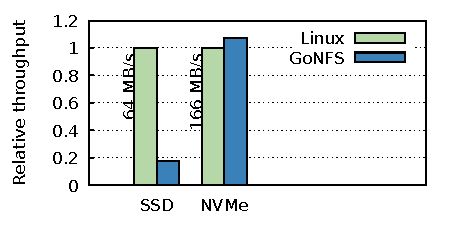
\includegraphics[scale=0.9]{fig/largefile-alt.pdf}
  \caption{Performance of \cc{largefile} depends on the storage medium. Linux
    takes advantage of unstable writes to write a large amount of data between
    barriers but \gnfs flushes to disk frequently.}
  %\caption{Performance of \cc{largefile} on a slow SSD across a few
  %  configurations. \tej{I wanted a cluster per configuration, and colors to
  %    correspond to the system.}}
\label{fig:largefile}
\end{figure}

% \begin{figure}[ht!]
%   \centering
%
%   \includegraphics[scale=0.9]{fig/aws/bench.pdf}
%
%   \caption{Performance of Linux NFS and \txn + \gnfs for \cc{smallfile},
%     \cc{largefile}, and \cc{app} workload, on a RAMdisk. \joe{This was run on an
%       AWS i3.metal with a Go in-memory disk.}}
% \label{fig:perf-aws}
% \end{figure}
%
% \begin{figure}[ht!]
%   \centering
%
%   \includegraphics[scale=0.9]{fig/aws/bench-ssd.pdf}
%
%   \caption{Performance of Linux NFS and \txn + \gnfs for \cc{smallfile},
%     \cc{largefile}, and \cc{app} workload, on a fast NVMe SSD. \joe{This was run
%       on an AWS i3.metal.}}
% \label{fig:perf-aws-ssd}
% \end{figure}

We first evaluate \gnfs's performance with a single client issuing requests.
\autoref{fig:perf} shows the results on the Intel Xeon desktop with both file systems backed by RAM, to
avoid any I/O overhead --- \gnfs takes a simple Go interface for the disk, which
we implemented with a large array, while ext4 uses a file in
tmpfs.\footnote{Running \gnfs on tmpfs performs slightly worse due to the around
  1 microsecond syscall overhead of each disk operation, which ext4
  does not incur since everything happens within the kernel.} \gnfs achieves at
least the throughput of ext4 across the different workloads.

On both the NVMe and slower SSD, \txn's performance relative to ext4 is similar on the \cc{smallfile} and \cc{app} workloads (not plotted),
again achieving at least 90\% of the throughout of ext4.
%
% next consider the effects of I/O overhead on disks. For the
% \cc{smallfile} and \cc{app} workloads, \txn's performance relative to ext4
% on both the NVMe and slower SSD is similar to ramdisk,
However, \gnfs performance on the \cc{largefile} benchmark is sensitive to disk I/O characteristics,
as shown in \autoref{fig:largefile}. On the faster NVMe device, \gnfs's large file performance
is comparable to ext4's, but on the slower SSD, it drops to under 20\% of ext4's throughput.
The reason is that the \cc{largefile}
benchmark produces a large number of parallel, unstable writes to the same file.
\gnfs runs them sequentially due to a per-inode lock, and then journals sequentially because it
ignores the unstable write flag. A disk barrier on the SSD takes about 2
milliseconds, so getting good disk throughput requires writing a large amount of
data before issuing a barrier, and the 64~KB batch size is insufficient to get
the maximum SSD write throughput. Re-running the experiment with
unstable writes enabled in \gnfs raises its throughput to 90\% of ext4's.

% The figure shows that \gnfs achieves
% comparable performance when using unstable writes, because even though the
% writes are issued sequentially \txn commits them to disk in large batches. Both
% systems get the same low performance if the benchmark is changed to consist of
% sequential, stable writes with the NFS client's \cc{sync} mount option, causing
% ext4's journaling behavior to match \gnfs in order to guarantee each write is
% persisted before the next is issued.

% shows the relative performance on this workload.

% \ralf{Are we switching to a different figure here?
% Namely Figure 19, which the comment says we will cut?}
% When run on a fast NVMe disk, relative
% performance is nearly identical. \tej{James suggested using the NVMe numbers as
% the main results and mentioning RAMdisk in passing.} \gnfs is able to achieve 90--95\% of the
% throughput of ext4 across the different workloads. We expect \gnfs and \txn to
% be somewhat slower, because they are written in Go rather than C, but \txn does
% implement sophisticated performance optimizations such as in-place updates of
% buffers, full-block overwrites without read-modify-write, etc. This suggests
% that \txn is a realistic journaling system for performant storage applications.
%
% On an SSD, \txn gets comparable performance for the \cc{smallfile} and \cc{app}
% benchmarks but is slower than Linux for the \cc{largefile} benchmark, as seen in
% \autoref{fig:perf-ssd} which shows relative throughput on the same benchmarks as
% \autoref{fig:perf} but on an SSD instead of a RAMdisk. We further explored the
% performance of this benchmark by running a number of other configurations, shown
% in \autoref{fig:largefile}. The \cc{largefile}
% benchmark produces a large number of parallel writes to the same file, which
% \gnfs runs sequentially due to a per-inode lock and journals sequentially due to
% the use of stable writes. The SSD can get 150 MB/s with sequential writes, but
% this requires writing a large amount of data before issuing a disk barrier,
% larger than the 64~KB write batch size. The figure shows that \gnfs achieves
% comparable performance when using unstable writes, because even though the
% writes are issued sequentially \txn commits them to disk in large batches. Both
% systems get the same low performance if the benchmark is changed to consist of
% sequential, stable writes with the NFS client's \cc{sync} mount option, causing
% ext4's journaling behavior to match \gnfs in order to guarantee each write is
% persisted before the next is issued.
% increasing the write batch size further to 128~KB also improves performance.

%\mfk{this paragraph doesn't have a clear narrative. it also seem to imply
%  that DFSQ has more CPU overhead because its implementation is more
%  sophisticated; i thought it was primarily due to Haskell}
%Compared with DFSCQ (a verified file system implemented by extracting Haskell
%code from Coq), \gnfs has equal or better performance, even with a single
%thread. We ran the same set of workloads to compare, and the only benchmark
%where DFSCQ has comparable performance is the in-memory \cc{smallfile} benchmark. For
%the other benchmarks and on an SSD, it obtains 40-60\% of the throughput (not
%plotted), even when DFSCQ is run through FUSE without the overhead of NFS. This
%is due to CPU overhead, since DFSCQ has a more sophisticated logging design than
%\gnfs that more aggressively buffers writes in memory. DFSCQ is single-threaded
%so with multiple concurrent clients throughput only gets worse.
%\tej{Do we want to put this in some plot, even if it's smaller? It's confusing
%to discuss results that aren't shown. Or, we may simplify our comparison to
%``it can be much worse and is never better''}

\subsection{\txn concurrency improves performance}
\label{sec:eval:concur}

To test whether the concurrency of \txn is important for performance we
measure the aggregate throughput of \gnfs with an increasing number of
clients that run the \cc{smallfile} benchmark.  We run the experiment
on a physical disk instead of an in-memory
file system so that while a thread is waiting for the disk another thread
can run.  We compare the performance of \gnfs to that of Linux ext4,
and to a single-threaded version of \gnfs that has no concurrency.

\autoref{fig:scale} shows the results on an EC2 i3.metal instance with an NVMe
SSD.  Both \gnfs and Linux ext4 take advantage of concurrent requests to
increase throughput.
The single-threaded \gnfs does just barely improve performance, from
parallelization among the clients and NFS server, but this amounts to less than
$2\times$ throughput with 20 clients than with one. Even with one client, \gnfs
achieves 35\% higher throughput than
single-threaded \gnfs due to concurrency between the RPC thread,
the logger thread, and the installer thread.  \gnfs achieves higher
throughput than Linux ext4, but it is hard to pin down the reason why,
because there are many differences in the designs.  One possibility
is that Linux ext4 does not have concurrent logging and installation
(but \txn does); another possibility is that ext4 waits for outstanding
transactions to finish before flushing to disk (but \txn does not).

\autoref{fig:scale-ssd} shows the scaling of \gnfs and Linux, this time on the Xeon desktop with a
slower SSD. While \gnfs obtains comparable performance for 7 or fewer cores,
Linux scales linearly beyond while \gnfs does not. The scaling in this case
primarily comes from batching writes from concurrent clients, resulting in
better disk write throughput.
\txn is not as careful about this, sometimes committing a small amount of data
rather than gathering many multi-writes and issuing them
together. The NVMe experiment in \autoref{fig:scale} uses storage with fast
enough random-write access that CPU efficiency is more important than issuing
large sequential writes; while a disk barrier takes 2 milliseconds on the SSD it
takes only 30 \emph{microseconds} on the NVMe disk.

\begin{figure}[ht!]
  \centering

  \includegraphics[scale=0.9]{fig/aws-spectre/scale.pdf}

  \caption{Combined throughput of multiple parallel \cc{smallfile}
    microbenchmarks, each creating files in different directories,
    on an NVMe SSD.}
  \label{fig:scale}
\end{figure}

\begin{figure}[ht!]
  \centering

  \includegraphics[scale=0.9]{fig/scale.pdf}

  \caption{Combined throughput of multiple parallel \cc{smallfile}
    microbenchmarks, each creating files in different directories,
    on a (slow) SSD.}
  \label{fig:scale-ssd}
\end{figure}

\subsection{Journaling atomicity simplifies proofs}
\label{sec:eval:atomic}

Many storage systems use journaling because they simplify the
implementation in terms of crash safety: the only point at which durable
state is modified is when an operation commits.  A goal of
\txn is to carry this insight into proofs, so that a storage system
using the journal can prove an operation is atomic using reasoning about durable
storage only at the commit point.

One measure of how well \txn achieves this goal is the lines of code in
\simplenfs that require reasoning about durable state.  \simplenfs
consists of \simplenfsLOC{} lines of verified code.  Only \simplenfsCrashLOC{} lines of code require
proofs to explicitly consider durable state, using crash conditions.
In \autoref{fig:write}, for example, crash reasoning is only needed for lines
6--8 when acquiring and releasing with the crash-aware lock specification.  All
of the other
code does not require reasoning about durable state; it suffices to prove
simple crash-free specifications that have a pre- and post-condition, but
no crash condition.  This formal reasoning is enabled by two techniques
from Perennial: lifting disk-object ownership and crash framing.

% \paragraph{Lifting disk-object ownership.}
% Lifting simplifies reasoning about disk-object ownership in \simplenfs in
% two ways.  First, lifting enables \simplenfs to transfer a predicate about
% disk-object ownership into a predicate about in-memory transaction state.
% Subsequent reads and writes within a transaction can operate on the
% transaction state, without worrying about durability until commit.
% Second, lifting enables \simplenfs to transfer predicates about
% disk-object ownership across crashes, to prove that on-disk state is
% correctly preserved on recovery.

% \paragraph{Framing the crash condition.}
% To formally prove that transactions are crash-safe, \simplenfs uses crash
% condition framing.  Specifically, when \simplenfs lifts some predicate
% into a transaction (e.g., a predicate describing the state of the inode),
% the proof immediately uses the durable disk-object ownership to frame
% away the crash-condition obligation until the commit point.  Using the
% durable resources to frame the crash obligation means that the durable
% resources are not available until commit, which in turn proves that they
% are not modified.  At commit time, the resources become available again,
% and the developer must explicitly reason about their crash safety (e.g.,
% just in the code shown in \autoref{fig:writecommit}).


\subsection{Perennial enables modular crash reasoning}
\label{sec:eval:modular}

Atomic crash specifications are crucial for enabling modular reasoning
about crash safety.  In \txn, atomic crash specs are used at many
layer boundaries.  Out of the layers shown in \autoref{fig:layers},
\textsc{circular}, \textsc{wal}, \textsc{obj}, and \textsc{jrnl} all
provide atomic crash specifications, which are used by the layer above. One benefit of atomic crash specs is that they
allowed us to develop these layers independently, using the specifications of
lower layers before their implements were fully proven, as one would
expect of any good API.

The modularity in Perennial largely follows the same structure as the code.
\autoref{fig:loc} shows that the \textsc{wal} and \textsc{jrnl} proofs were
split into an atomic transition specification about the code and a proof-only
abstraction on top, but the bulk of the division was due to boundaries in the
code that made the implementation manageable. Using separation logic it was easy
to prove data structures (like the striped lockmap) and individual utility
functions and use their abstract specifications elsewhere in the proof.

\subsection{Proof effort}
\label{sec:eval:proof}

\autoref{fig:loc} shows the lines of code and lines of proof for \txn
and \simplenfs.  The hardest part of \txn lies in the \textsc{wal}
layer, which has significant lock-free concurrency, and requires careful
reasoning about crashes and recovery.  This is reflected in \textsc{wal}'s
relatively high lines of code, lines of proof, and proof:code ratio.
In contrast,
\simplenfs leverages GoJournal's atomicity, and ends up with a
much smaller proof relative to its code size.


\subsection{Verification prevents bugs}
\label{sec:eval:bugs}

% When developing \simplenfs and
% \txn, we wrote extensive unit tests, but they were not sufficient to
% find all bugs before proving.  When proving \simplenfs, we discovered
% several bugs due to uncaught integer overflows (which wrap around in Go) and
% out-of-bounds reads and writes that could have led to file-system corruption
% (e.g., if the write RPC includes an offset and count that, if added together in
% 64-bit arithmetic, overflows to a value less than the current size of
% the file).

When developing \txn, we wrote unit tests to quickly find problems before starting
verification, but they did not catch all bugs. While proving
\txn, we found a subtle bug in absorption.  When appending a new
transaction in memory, \txn has an optimization called absorption where earlier
writes to the same address are replaced with the new values. However, we discovered a race condition,
where the logger thread could have been already flushing those earlier
writes to disk, leading to unpredictable disk contents depending on the
order of absorption vs logging.  We fixed this issue by introducing the
\cc{nextDiskEnd} boundary, as shown in \autoref{fig:log}: the logger thread only
logs up to \cc{nextDiskEnd}, and absorption is only allowed to modify values
after \cc{nextDiskEnd}.


% Caught a bug where a variable got changed and then we read the new value: \url{https://github.com/mit-pdos/goose-nfsd/commit/255a1c4cc}.
% Forgot to check for out-of-bounds: \url{https://github.com/mit-pdos/goose-nfsd/commit/5cb7b82b9c809}
% Couple missing overflow checks: \url{https://github.com/mit-pdos/goose-nfsd/commit/f5d41e3926c2}, \url{https://github.com/mit-pdos/goose-nfsd/commit/31cc9dcc1}
% Check for inode read past end: \url{https://github.com/mit-pdos/goose-nfsd/commit/b91113936d27}
% added an optimization to make the proof easier: \url{https://github.com/mit-pdos/goose-nfsd/commit/a788305ba0d7}
% introduced data structure (sliding) for mem log to make verification more modular
% introduced layer for on-disk circular log to make verification more modular

% \mfk{describe trusted computing base somewhere: here or in system overview?}

\section{Conclusion}
\label{sec:concl}

\txn is the first concurrent crash-safe journaling
system with a machine-checked proof, built on top of the Perennial 2.0 framework.
\txn uses Perennial's techniques, including lifting and crash framing, to
carry over the atomic benefits of journaling to its formal specification.
This enables storage applications to use mostly crash-free reasoning in
their proofs.  For example, in the verified \simplenfs server, only \simplenfsCrashLOC{}
lines of code, out of \simplenfsLOC{}, required crash reasoning.  \txn is sophisticated
enough to implement a functional (but unverified) NFSv3 server, \gnfs, that achieves
90\% of the performance of a Linux ext4 NFSv3 server on a development workload, far higher than
any previous verified file systems, and \txn's concurrency enables \gnfs
to scale with concurrent client requests.  To simplify \txn's proofs,
Perennial provides logically atomic crash specifications, which capture the
crash properties of internal interfaces as single logical transitions,
enabling modular proofs for \txn's internal layers.

